% This is the Reed College LaTeX thesis template. Most of the work 
% for the document class was done by Sam Noble (SN), as well as this
% template. Later comments etc. by Ben Salzberg (BTS). Additional
% restructuring and APA support by Jess Youngberg (JY).
% Your comments and suggestions are more than welcome; please email
% them to cus@reed.edu
% 
% See http://web.reed.edu/cis/help/latex.html for help. There are a 
% great bunch of help pages there, with notes on
% getting started, bibtex, etc. Go there and read it if you're not
% already familiar with LaTeX.
% 
% Any line that starts with a percent symbol is a comment. 
% They won't show up in the document, and are useful for notes 
% to yourself and explaining commands. 
% Commenting also removes a line from the document; 
% very handy for troubleshooting problems. -BTS

% As far as I know, this follows the requirements laid out in 
% the 2002-2003 Senior Handbook. Ask a librarian to check the 
% document before binding. -SN

%% 
%% Preamble
%% 
% \documentclass{<something>} must begin each LaTeX document
\documentclass[12pt,twoside]{reedthesis}
% Packages are extensions to the basic LaTeX functions. Whatever you
% want to typeset, there is probably a package out there for it.
% Chemistry (chemtex), screenplays, you name it.
% Check out CTAN to see: http://www.ctan.org/
%% 
\usepackage{graphicx,latexsym} 
\usepackage{amssymb,amsthm,amsmath}
\usepackage{longtable,booktabs,setspace}
\usepackage{braket}
\usepackage{mathtools}
\usepackage[hyphens]{url}
\usepackage{rotating}
\usepackage{ytableau}
\usepackage[capitalise]{cleveref}
\usepackage{algpseudocodex}
\usepackage{setspace}
%\usepackage[noadjust]{cite}
% make notes fit in margins
\usepackage{todonotes}
\usepackage{url}
\setlength{\marginparwidth}{2cm}
\usepackage{tikz}
\usetikzlibrary{quantikz2}
\usepackage{float}
% make paragraphs nicer
% \usepackage[skip=40pt plus1pt, indent=40pt]{parskip}

% \usepackage{natbib}
%usepackage[numbers]{natbib}
\usepackage[style=numeric,backend=biber,useprefix=false,sortcites=true]{biblatex}
\addbibresource{thesisnew.bib}

\usepackage[final]{microtype}

% Comment out the natbib line above and uncomment the following two lines to use the new 
% biblatex-chicago style, for Chicago A. Also make some changes at the end where the 
% bibliography is included. 
% \usepackage{biblatex-chicago}
% \bibliography{thesis}

% other fonts are available like times, bookman, charter, palatino
% \usepackage[cmintegrals,cmbraces]{newtxmath}
% \usepackage{ebgaramond-maths}
% \usepackage[T1]{fontenc}
% beware, math preamble paste begins



\theoremstyle{plain}   % This is the default, anyway
\newtheorem{thm}{Theorem}[section] % numbered theorem
\makeatletter\let\c@thm\c@thm\makeatother
\newtheorem{cor}{Corollary}[section]
\makeatletter\let\c@cor\c@thm\makeatother
\newtheorem{lemma}{Lemma}[section]
\makeatletter\let\c@lemma\c@thm\makeatother
\newtheorem{prop}{Proposition}[section]
\makeatletter\let\c@prop\c@thm\makeatother
\newtheorem{claim}{Claim}[section]
\makeatletter\let\c@claim\c@thm\makeatother
\newtheorem{conj}{Conjecture}[section]
\makeatletter\let\c@conj\c@thm\makeatother

\newtheorem*{unnumberedtheorem}{Theorem}  % unnumbered theorem
\newtheorem*{unnumberedcorollary}{Corollary}
\newtheorem*{unnumberedlemma}{Lemma}
\newtheorem*{unnumberedproposition}{Proposition}
\newtheorem*{unnumberedclaim}{Claim}

\theoremstyle{definition}

\newtheorem{defn}{Definition}[section]
\makeatletter\let\c@defn\c@thm\makeatother
\newtheorem{const}{Construction}[section]
\makeatletter\let\c@const\c@thm\makeatother
\newtheorem{notn}{Notation}[section]
\makeatletter\let\c@notn\c@thm\makeatother
\newtheorem{outline}{Proof Outline}[section]
\makeatletter\let\c@outline\c@thm\makeatother
\newtheorem{post}{Postulate}[section]
\makeatletter\let\c@outline\c@thm\makeatother


\theoremstyle{remark}

\newtheorem{rem}{Remark}[section]
\makeatletter\let\c@rem\c@thm\makeatother
\newtheorem{ex}{Example}[section]
\makeatletter\let\c@ex\c@thm\makeatother
\newtheorem{observation}{Observation}[section]
\makeatletter\let\c@observationn\c@thm\makeatother

\newtheorem*{unnumberedtheoremremark}{Remark}
\newtheorem*{unnumberedtheoremexample}{Example}
\newtheorem*{unnumberedtheoremdefinition}{Defintion}

\makeatletter
\let\c@equation\c@thm
\numberwithin{equation}{section}
\makeatother

\def\cA{\mathcal{A}}\def\cB{\mathcal{B}}\def\cC{\mathcal{C}}\def\cD{\mathcal{D}}\def\cE{\mathcal{E}}\def\cF{\mathcal{F}}\def\cG{\mathcal{G}}\def\cH{\mathcal{H}}\def\cI{\mathcal{I}}\def\cJ{\mathcal{J}}\def\cK{\mathcal{K}}\def\cL{\mathcal{L}}\def\cM{\mathcal{M}}\def\cN{\mathcal{N}}\def\cO{\mathcal{O}}\def\cP{\mathcal{P}}\def\cQ{\mathcal{Q}}\def\cR{\mathcal{R}}\def\cS{\mathcal{S}}\def\cT{\mathcal{T}}\def\cU{\mathcal{U}}\def\cV{\mathcal{V}}\def\cW{\mathcal{W}}\def\cX{\mathcal{X}}\def\cY{\mathcal{Y}}\def\cZ{\mathcal{Z}}

\def\AA{\mathbb{A}} \def\BB{\mathbb{B}} \def\CC{\mathbb{C}} \def\DD{\mathbb{D}} \def\EE{\mathbb{E}} \def\FF{\mathbb{F}} \def\GG{\mathbb{G}} \def\HH{\mathbb{H}} \def\II{\mathbb{I}} \def\JJ{\mathbb{J}} \def\KK{\mathbb{K}} \def\LL{\mathbb{L}} \def\MM{\mathbb{M}} \def\NN{\mathbb{N}} \def\OO{\mathbb{O}} \def\PP{\mathbb{P}} \def\QQ{\mathbb{Q}} \def\RR{\mathbb{R}} \def\SS{\mathbb{S}} \def\TT{\mathbb{T}} \def\UU{\mathbb{U}} \def\VV{\mathbb{V}} \def\WW{\mathbb{W}} \def\XX{\mathbb{X}} \def\YY{\mathbb{Y}} \def\ZZ{\mathbb{Z}}  

\def\fa{\mathfrak{a}} \def\fb{\mathfrak{b}} \def\fc{\mathfrak{c}} \def\fd{\mathfrak{d}} \def\fe{\mathfrak{e}} \def\ff{\mathfrak{f}} \def\fg{\mathfrak{g}} \def\fh{\mathfrak{h}} \def\fj{\mathfrak{j}} \def\fk{\mathfrak{k}} \def\fl{\mathfrak{l}} \def\fm{\mathfrak{m}} \def\fn{\mathfrak{n}} \def\fo{\mathfrak{o}} \def\fp{\mathfrak{p}} \def\fq{\mathfrak{q}} \def\fr{\mathfrak{r}} \def\fs{\mathfrak{s}} \def\ft{\mathfrak{t}} \def\fu{\mathfrak{u}} \def\fv{\mathfrak{v}} \def\fw{\mathfrak{w}} \def\fx{\mathfrak{x}} \def\fy{\mathfrak{y}} \def\fz{\mathfrak{z}}
\def\fN{\mathfrak{N}}
\def\fgl{\mathfrak{gl}}  \def\fsl{\mathfrak{sl}}  \def\fso{\mathfrak{so}}  \def\fsp{\mathfrak{sp}}  
\def\GL{\mathrm{GL}} \def\SL{\mathrm{SL}}  \def\SP{\mathrm{SL}}\def\OG{\mathrm{O}}

\def\aa{\mathbf{a}} \def\bb{\mathbf{b}} \def\cc{\mathbf{c}} \def\dd{\mathbf{d}} \def\ee{\mathbf{e}} \def\ff{\mathbf{f}}
% \def\gg{\mathbf{g}}
\def\hh{\mathbf{h}} \def\ii{\mathbf{i}} \def\jj{\mathbf{j}} \def\kk{\mathbf{k}}
% \def\ll{\mathbf{l}}
\def\mm{\mathbf{m}} \def\nn{\mathbf{n}} \def\oo{\mathbf{o}} \def\pp{\mathbf{p}} \def\qq{\mathbf{q}} \def\rr{\mathbf{r}} \def\ss{\mathbf{s}}  \def\uu{\mathbf{u}} \def\vv{\mathbf{v}} \def\ww{\mathbf{w}} \def\xx{\mathbf{x}} \def\yy{\mathbf{y}} \def\zz{\mathbf{z}}
\def\zzero{\mathbf{0}}

\def\<{\langle} \def\>{\rangle}
\def\Aut{\mathrm{Aut}}
\def\ch{ \stackrel}
\def\col{\mathrm{col}}
\def\dim{\mathrm{dim}} 
\def\End{\mathrm{End}} 
\def\ev{\mathrm{ev}} 
\def\f{\varphi}
\def\gcd{\mathrm{gcd}}
\def\half{\hbox{$\frac12$}}
\def\Hom{\mathrm{Hom}}
\def\Sym{\mathrm{Sym}}
\def\img{\mathrm{img}}
\def\id{\mathrm{id}} 
\def\Inn{\mathrm{Inn}}
\def\lcm{\mathrm{lcm}}
\def\normeq{\trianglelefteq}
% \def\ch{ \stackrel{\mathrm{ch}}{\trianglelefteq}}
% \def\normeq{\trianglelefteq}
\def\nul{\mathrm{nullity}}
\def\row{\mathrm{row}}
\def\rk{\mathrm{rank}}
\def\sgn{\mathrm{sgn}}
\def\sp{\mathrm{span}}
\def\supp{\mathrm{supp}}
\def\Syl{\mathrm{Syl}}
\def\tr{\mathrm{tr}} 
\def\vep{\varepsilon}

\def\ind{\mathrm{Ind}}
\def\res{\mathrm{Res}}
\def\irr{\mathrm{Irr}}
\def\stab{\mathrm{Stab}}
\def\prob{\mathrm{Prob}}
% \usepackage{mathabx}
\def\acts{\circlearrowright} %group action

% Cleveref definitions
% \crefname{lemma}{Lemma}{Lemmas}
% \crefname{thm}{Theorem}{Theorems}
% \crefname{defn}{Definition}{Definitions}
% \crefname{notn}{Notation}{Notations}
% \crefname{const}{Construction}{Constructions}
% \crefname{prop}{Proposition}{Propositions}
% \crefname{rem}{Remark}{Remarks}
% \crefname{cor}{Corollary}{Corollaries}
% \crefname{equation}{Diagram}{Diagrams}
% \crefname{ex}{Example}{Examples}

% Arrays:
\newcommand\Pmatrix[1]{\begin{pmatrix}#1\end{pmatrix}}
\newcommand\smatrix[1]{\text{\small$\begin{pmatrix}#1\end{pmatrix}$}}
\newcommand\fmatrix[1]{\text{\footnotesize$\begin{pmatrix}#1\end{pmatrix}$}}
\newcommand\tmatrix[1]{\text{\tiny$\begin{pmatrix}#1\end{pmatrix}$}}

\DeclarePairedDelimiter\ceil{\lceil}{\rceil}
\DeclarePairedDelimiter\floor{\lfloor}{\rfloor}
% math preamble ends






\title{Two Cases of the Symmetric Oracle Discrimination Problem: Representation Theory in Quantum Computing}
\author{Dale D. Schandelmeier-Lynch}
% The month and year that you submit your FINAL draft TO THE LIBRARY (May or December)
\date{May 2025}
\division{Mathematical and Natural Sciences}
\advisor{Jamie Pommershiem}
% If you have two advisors for some reason, you can use the following
\altadvisor{Greg Anderson}
%%% Remember to use the correct department!
\department{Mathematics and Computer Science}
% if you're writing a thesis in an interdisciplinary major,
% uncomment the line below and change the text as appropriate.
% check the Senior Handbook if unsure.
\thedivisionof{The Established Interdisciplinary Committee for}
% if you want the approval page to say "Approved for the Committee",
% uncomment the next line
\approvedforthe{Committee}

\setlength{\parskip}{0pt}
%% 
%% End Preamble
%% 
%% The fun begins:
\begin{document}

  \maketitle
  \frontmatter % this stuff will be roman-numbered
  \pagestyle{empty} % this removes page numbers from the frontmatter

% Acknowledgements (Acceptable American spelling) are optional
% So are Acknowledgments (proper English spelling)
  \chapter*{Acknowledgements}

  I greatly appreciate Zajj Daugherty's help with the decomposition of $\CC \Omega_k$ via Young's rule and also for several enlightening discussions.
  Additionally, some of Zajj's ideas are offered in the discussion section as potential clues for future proofs in this area.
  
  \bigskip
  I would also like to thank Jamie and Greg for being helpful advisors and for keeping me on track to finish my thesis on time.
  
  \bigskip
  One of the papers I cite often by Cohen De Valle was introduced to me by Daniel Copeland via Jamie; that input is what gave my thesis a solid direction to work in.

  \bigskip
  Finally, I would like to thank my family for encouraging me and supporting me in my education.
  % The preface is optional
  % To remove it, comment it out or delete it.
  % \chapter*{Preface}
  % This is an example of a thesis setup to use the reed thesis document class.



  % \chapter*{List of Abbreviations}
  % You can always change the way your abbreviations are formatted. Play around with it yourself, use tables, or come to CUS if you'd like to change the way it looks. You can also completely remove this chapter if you have no need for a list of abbreviations. Here is an example of what this could look like:

  % \begin{table}[h]
  %   \centering % You could remove this to move table to the left
  %   \begin{tabular}{ll}
  %     \textbf{ABC}  	&  American Broadcasting Company \\
  %     \textbf{CBS}  	&  Columbia Broadcasting System\\
  %     \textbf{CDC}  	&  Center for Disease Control \\
  %     \textbf{CIA}  	&  Central Intelligence Agency\\
  %     \textbf{CLBR} 	&  Center for Life Beyond Reed\\
  %     \textbf{CUS}  	&  Computer User Services\\
  %     \textbf{FBI}  	&  Federal Bureau of Investigation\\
  %     \textbf{NBC}  	&  National Broadcasting Corporation\\
  %   \end{tabular}
  % \end{table}


  \tableofcontents
  % % if you want a list of tables, optional
  % \listoftables
  % % if you want a list of figures, also optional
  % \listoffigures

  \mainmatter % here the regular arabic numbering starts
  \pagestyle{fancyplain} % turns page numbering back on

  % The abstract is not required if you're writing a creative thesis (but aren't they all?)
  % If your abstract is longer than a page, there may be a formatting issue.
  \chapter*{Abstract}
  
  % Quantum mechanics and quantum computing are introduced, along with representation theory in general and for the symmetric group.
  % The question of symmetric oracle discrimination, where an algorithm queries $G$-set elements $\omega$ to receive $g \cdot \omega$ to solve for $g$,
  % is defined formally for $S_n$ acting naturally on $\{K \subseteq [n] | |K| = k\}$ and $\{P \vdash [n] | |P| = b, |p| = a \forall p \in P\}$.
  % Work in \cite{copeland} allows for the reduction of the quantum oracle question to one of representation theory.
  % Via GAP the quantum query complexity is explicitly computed for small $G$-sets.
  % Various conjectures are formed, the broadest being that any permutation group $G$ admitting a base-controlling homomorphism has equivalent quantum and classical query complexity for symmetric oracle discrimination.
  % When $S_k \acts \{K \subseteq [n] | |K| = 2k\}$, we prove that the quantum and classical query complexities are equal.
  
  Quantum mechanics and quantum computing are introduced, along with representation theory both in general and for the symmetric group.
  The problem of symmetric oracle discrimination, where an algorithm queries $G$-set elements $\omega$ to receive $g \cdot \omega$ to solve for $g$,
  is defined formally for $S_n$ acting naturally on $k$-element subsets of $[n]$ and regular partitions of $[n]$ into $b$ parts of size $a$.
  Recent work from Copeland and Pommershiem allowed for the reduction of the coset identification problem, a generalized symmetric oracle discrimination, to one of representation theory.
  Using the GAP programming language and representation theory, the quantum query complexity is explicitly computed for small $G$-sets.
  Various conjectures are formed from this data, the broadest being that any permutation group $G$ admitting a base-controlling homomorphism has equivalent quantum and classical query complexity for symmetric oracle discrimination.
  When $S_{2k}$ is acting on the set of $k$ element subsets of $[2k]$ in symmetric oracle discrimination, we prove that the quantum and classical query complexities are equal.
  \onehalfspacing
  % \doublespacing



  \chapter*{Introduction}
  \addcontentsline{toc}{chapter}{Introduction}
  \chaptermark{Introduction}
  \markboth{Introduction}{Introduction}

  Theoretical quantum computing often employs a model %\todo{maybe this shouldn't be called a model}
  of asymptotic analysis known as \emph{oracle problems} as an abstraction to make comparisons between classical and quantum computers easier.
  An oracle is a theoretical function whose inner workings cannot be observed or manipulated; algorithms are only allowed to choose an input to the oracle and receive its output.
  The goal when given an oracle problem is to create an algorithm which learns a given characteristic of the function hidden by the oracle.
  We usually assume that the function hidden by the oracle is sampled randomly from a distribution known to the algorithm.
  A simple example is as follows. For a function $f: \{a_0, a_1 \} \to \ZZ / 2\ZZ$ uniformly sampled from the space of possible functions, determine the mod $2$ sum $a_0 \oplus a_1$.
  Here we define the oracle $O$ to offer information to the algorithm through the black-box function $O(x) \coloneq f(x)$.
  A classical algorithm would have to make $2$ queries to $O$ for exact learning, as it must query every element of the codomain to learn the values of $a_0$ and $a_1$.
  As it turns out, a well-known quantum algorithm called Deutsch's algorithm can learn the value of $a_0 \oplus a_1$ with certainty after just $1$ query! \par
  Also of interest in oracle problems is \emph{bounded-error} learning, where we consider how many queries are needed until an algorithm has some $\geq \frac{2}{3}$ chance of guessing the characteristic correctly.
  Contrast the previous example with a problem where the algorithm has to learn $f$ exactly; before making any queries the classical algorithm has a $\frac{1}{2}$ chance of guessing $a_0 \oplus a_1$ correctly,
  and this doesn't change after making a query. On the other hand, learning the exact function has a $\frac{1}{4}$ chance of success with $0$ queries, and a $\frac{1}{2}$ chance of success with $1$ query.
  If we considered an extreme version of this problem, $f: \{a_0, a_1 \} \to \ZZ / 1000\ZZ$, then we observe that a classical algorithm has a near-zero chance of guessing the function before it makes its final query.
  For many oracle problems, this pattern holds true in the classical case; the algorithm knows nearly nothing about the function until it knows the whole function.
  Effectively, bounded-error learning is equivalent to exact learning classically. \par
  Shockingly, quantum algorithms have a different tendency.
  The function will be nearly unknown for the first few queries, but after an asymptotically %\todo{maybe this asymptotic claim is false}
  smaller number of queries than those needed for exact learning, nearly the whole function will be known!
  We are thus concerned with comparing the exact classical query complexity with both the exact and bounded-error quantum query complexity of a given oracle problem.
  Of note is that if we find a proof using our methods, we have found a necessary and sufficient number of queries to solve the problem;
  we prove the existence of an algorithm which solves the problem with the given asymptotics, and it is optimal,
  meaning no algorithm makes asymptotically fewer queries.
  % In fact, we will be able to prove that there exists an algorithm which has a given query complexity, and that furthermore no algorithm exists which can do better --- the algorithm will be optimal.
  \par
  Our oracle problem comes from \cite{copeland}, as a specification of the more general coset identification problem:
  Suppose a group $G$ acts by permutations on a finite set $\Omega$ (we call $\Omega$ a $G$-set).
  An algorithm is given access to an oracle which takes an element $\omega \in \Omega$ and returns $a \cdot \omega$ for some hidden group element (uniformly sampled) $a \in G$. The goal is to guess
  the hidden element $a \in G$.
  We will be concerned with the groups $S_n$ and $A_n \leq S_n$ acting on the set of $k$ element subsets of $n$, and on the set of regular partitions of $n$ into $b$ parts of size $a$.
  \par
  To answer these problems we will use a crucial result from \cite{copeland} which enables us to determine optimal quantum query complexity with a correspondence.
  Taking the tensor product of a representation derived from our $G$-set $\Omega$ with itself repeatedly will be equivalent to making oracle queries, turning our quantum computing problem
  into one of representation theory.
  By understanding the representation corresponding to $\Omega$ and the way it tensors with itself, we will be able to find the query complexity.
  Because our $G$-sets have $S_n$ and $A_n$ as groups, we will be deeply concerned with the representation theory of $S_n$;
  combinatorial structures known as \emph{Young diagrams} and \emph{Young tableaux} will offer a useful correspondence through which we can understand $S_n$'s representations.
  
  
  \chapter{Background}
  We first introduce the necessary quantum computing and representation theory background to understand the problem statement in context.
  \section{Quantum Computing}
  Quantum computing utilizes the nonclassical nature of quantum mechanics to achieve asymptotic improvements over classical algorithms.
  Not all problems admit a quantum ``speedup''; we will be more specific about our computational framework after the necessary background.
  To illuminate the physical-mathematical framework in which quantum computing takes place, we will expound the postulates of quantum mechanics and the associated linear algebra from \cite[Chapter 2]{nielsen2010}.
  \subsection{Quantum Mechanics}
  Due to theorem 4.2 from \cite{copeland}, it turns out that our results rely almost entirely on representation theory;
  nevertheless we introduce the four fundamental postulates from \cite[Chapter 2]{nielsen2010} to provide context for the quantum model of computation. We will also rely on Nielsen and Chuang for standard definitions here.
  Throughout this section we use the ``bra-ket'' (or Dirac) notation to represent vectors in vector spaces. This is inherited from physics and uses the symbols
  $\ket{\cdot}$ called ket, $\bra{\cdot}$ called bra, and $\braket{\cdot | \cdot}$ called braket (as we have ``bracketed'' the symbols); 
  \[ \ket{\psi} \]
  is a vector we have labeled $\psi$. In quantum computing we are concerned with complex vector spaces by postulate; we need to define inner products both for this postulate and to elaborate on bra-ket notation.
  \begin{defn}[{Inner product}]
    A function $(\cdot, \cdot): V \times V \to \CC$ is a (complex) inner product if it satisfies the following requirements:
    \begin{enumerate}
    \item $(\cdot, \cdot)$ is linear in the second argument:
      \[ \left( \ket{v}, \sum_i \lambda_i \ket{w_i} \right) = \sum_i \lambda_i \left( \ket{v}, \ket{w_i} \right).\]
    \item $(\ket{v}, \ket{w}) = (\ket{v}, \ket{w})^*$.
    \item $(\ket{v}, \ket{v}) \geq 0$ with equality if and only if $\ket{v} = 0$.
    \end{enumerate}
  \end{defn}
  The intuition of braket notation is that $\bra{\phi}$ is the dual of the vector $\ket{\phi}$, which in the corresponding matrix presentation
  of vectors corresponds to turning a column vector into a row vector by taking its conjugate transpose. Therefore taking the standard matrix product
  \[\bra{\phi} \ket{\psi}\]
  is equivalent to the standard inner product $(\ket{\phi}, \ket{\psi}) = \sum_{k=1}^n \phi_k^* \psi_k$, which we notate as
  \[\braket{\phi | \psi};\]
  here the symbol $\cdot^*$ denotes the unary complex conjugation operation.
  The elegance of braket notation, aside from saving space, is that we can easily tell the output of complicated linear expressions.
  It's easy to see that $\braket{\phi | \psi} \braket{x | y} \in \FF$, while it takes a little thinking to see that
  \[
    \begin{bmatrix}
      x & y
    \end{bmatrix}
    \begin{bmatrix}
      x \\ y
    \end{bmatrix}
    \begin{bmatrix}
      x & y
    \end{bmatrix}
    \begin{bmatrix}
      x \\ y
    \end{bmatrix}
  \]
  equals a scalar.
  \par
  We are now ready to introduce our first postulate. As mathematicians we needn't worry about how physicists experimentally constructed these postulates, although their
  (approximate) truth will be necessary if we are to physically realize quantum computers and employ the algorithms we design.
  If we take these postulates at face value, phenomena that are strange from a classical physics standpoint feel like natural consequences of the mathematics;
  in that sense it can be helpful to abstract away your physical intuition and instead focus on the consequences of these postulates when we start doing computation.
  \begin{post}[{\cite[2.2.1]{nielsen2010}}]
    Associated to any isolated physical system is a complex vector space
    with inner product (that is, a Hilbert space) known as the \emph{state space} of the
    system. The system is completely described by its \emph{state vector}, which is a unit
    vector in the system's state space.
  \end{post}
  Here unit vector refers to a vector with norm $1$; the standard norm we employ is $|| \ket{\psi} || \coloneq \sqrt{\braket{\psi| \psi}}$.
  Note that quantum mechanics doesn't tell us the state space or state vector of a particular system; it only describes in general the characteristics systems share.
  In our quantum computing model we regard these physical systems as memory and perform operations on this memory through the appropriate mathematical morphism, which in this case are linear operators.
  A minor detail is that Hilbert spaces have more properties when they are infinite-dimensional, but in our case we will only ever use finite memory and so our Hilbert spaces are always finite-dimensional. \par
  The simplest quantum mechanical system is the \emph{qubit}. A qubit resides in $\CC^2$ and so has a two-dimensional state space.
  We use $\ket{0}$ and $\ket{1}$ to label the elements of an orthonormal basis for the qubit; in practice we let
  \[\ket{0} =
    \begin{pmatrix}
      1 \\
      0
    \end{pmatrix},
    \quad
    \ket{1} =
    \begin{pmatrix}
      0 \\
      1
    \end{pmatrix}.
  \]
  Note that $\ket{0}$ is not the zero vector $0$; we use $\ket{0}$ despite this overlap in reference to the two states of a bit, $0$ and $1$.
  What makes the qubit interesting in contrast is that we are not limited to state vectors $\ket{0}$ and $\ket{1}$; we know from linear algebra that
  we can express any element of the state basis as
  \[\ket{\psi} = a \ket{0} + b \ket{1}, \]
  where $a$ and $b$ are in the complex numbers. The state of the qubit is described by four real numbers (that is $x +iy$ where $x,y \in \RR$ for both $a$ and $b$) instead of one bit!
  A qubit can take on far more values than a bit because it can exist in a superposition of the states $\ket{0}$ and $\ket{1}$; that is both $a$ and $b$ can be nonzero at the same time.
  However, there is redundancy in this description due to the unit vector condition and relative phase; the qubit's state is in fact parameterized by a point on the surface of a three dimensional sphere, known as the \emph{Bloch sphere}.
  In our case we will be using the state space $\CC \Omega$ with standard basis $\{ \ket{\omega} | \omega \in \Omega\}$; you can imagine we have defined an abelian group structure on $\Omega$ and so we are
  considering the group algebra $\CC \Omega$ by linearization. \par
  We are now ready for our next postulate:
  \begin{post}[{\cite[2.2.2]{nielsen2010}}]
    The evolution of a \emph{closed} quantum system is described by a \emph{unitary transformation}. That is, the state $\ket{\psi}$ of the system at time $t_1$ is related to the state
    $\ket{ \psi^{'} }$ of the system at time $t_2$ by a unitary operator $U$ which depends only on the times $t_1$ and $t_2$;
    \[ \ket{\psi^{'}} = U \ket{\psi}.\]
  \end{post}
  With operators we can define the last piece of the bra-ket puzzle. If we consider the vector $\ket{v}$ from a Hilbert space $V$, and the vector $\ket{w}$ from a Hilbert space $W$,
  then we define the outer product notation for a linear operator $\ket{w} \bra{v} : V \to W$ as
  \[ (\ket{w} \bra{v}) (\ket{v^{'}}) \coloneq \ket{w} \braket{v|v^{'}} = \braket{v|v^{'}} \ket{w}.\]
  We can thus interpret the notation $\ket{w} \braket{v|v^{'}}$ in two ways: as a linear operator fed $\ket{v^{'}}$, and as the vector $\ket{w}$ scaled by the inner product of $\braket{v|v^{'}}$.
  In terms of matrix multiplication we see here the associativity property at work; the product of the column and row vectors $\ket{w} \bra{v}$ creates a matrix which then acts as a linear operator on
  $\ket{v^{'}}$, or the product of row and column vectors creates a scalar which then scales $\ket{w}$.
  \par
  To define a unitary operator, we first need the \emph{adjoint} or \emph{Hermitian conjugate} (\cite[2.1.6]{nielsen2010}) of an operator.
  This is the unique operator $A^\dag$ such that for all vectors $\ket{v_1}, \ket{v_2} \in V$,
  \[(\ket{v_1}, A \ket{v_2}) = ( A^\dag \ket{v_1}, \ket{v_2} ).\]
  Here the operation is the inner product; by convention we define $(\ket{v})^\dag \coloneq \bra{v}$ so that $(A \ket{v_1})^\dag \ket{v_2} = \braket{v_1 | A^\dag |v_2 }$.
  When we have a matrix representing an operator $A$, the standard definition of the adjoint is to take the conjugate and then the transpose of $A$: $A^\dag \coloneq (A^*)^T$.
  When $A^\dag = A$, we call $A$ \emph{Hermitian} or \emph{self-adjoint}.
  As a broader class we say that an operator $A$ is \emph{normal} if $AA^\dag = A^\dag A$; it is immediate that Hermitian operators are normal.
  Finally, we say an operator $U$ is unitary if $U^\dag U = I$, where $I$ is the identity operator (or matrix); for finite vector spaces it can be proven that this implies $ U U^\dag = I$, so unitary
  operators are also normal.
  We care about unitary products because they preserve inner products; observe that
  \begin{align*}
    & (U \ket{v}, U \ket{w}) = \braket{v | U^\dag U  | w} = \braket{v | I | w} = \braket{v | w}  & & \text{(\cite[2.36]{nielsen2010}).}
  \end{align*}


  Postulate 2 demands that operators be unitary so that the unit condition of the state vector is maintained. \par
  We are now ready for Postulate 3, which tells us what happens when an isolated quantum system is measured.
  To measure a quantum system it must be exposed to an external physical system, and so the rule of unitary evolution from Postulate 2 no longer necessarily applies.
  \begin{post}[{\cite[2.2.3]{nielsen2010}}]
    Quantum measurements are described by a collection $\{M_m\}$ of \emph{measurement operators}.
    These are operators acting on the state space of the system being measured.
    The index $m$ refers to the measurement outcomes that may occur in the experiment.
    If the state of the quantum system is $\ket{\psi}$ immediately before the measurement then the probability that result $m$ occurs is given by
    \[ p(m) = \braket{ \psi | M_m^\dag M_m | \psi},\]
    and the state of the system after the measurement is
    \[ \dfrac{M_m \ket{\psi}}{\sqrt{\braket{\psi | M_m^\dag M_m | \psi}}}.\]
    The measurement operators satisfy the \emph{completeness equation},
    \[ \sum_m M_m^\dag M_m = I.\]
    The completeness equation expresses the fact that probabilities sum to one:
    \[ 1 = \sum_m p(m) = \sum_m \braket{\psi | M_m^\dag M_m | \psi}.\]
  \end{post}
  The takeaways from this postulate are twofold. Measurements in a quantum system can change the state of the state vector; information can be lost by performing a measurement.
  From the real numbers contained in a state vector --- three in the case of the qubit --- we can only observe a finite number of states.
  In fact, if we are trying to distinguish between states that are not orthonormal, then we lose the guarantee of distinguishability.
  Because some state $\ket{\psi}$ is not orthonormal to some other distinct state $\ket{\phi}$, there is a component of $\ket{\psi}$ that is orthogonal to $\ket{\phi}$ and a component
  that is parallel to $\ket{\phi}$; therefore when you measure a system with state vector $\ket{\psi}$ there is a nonzero chance of it being misidentified as $\ket{\phi}$.
  This means that we can only perfectly distinguish between a number of states up to the dimension of the state space.
  Furthermore, cascaded measurements $\{L_l \}$ and $\{M_m\}$ are equivalent to a single measurement with operators $\{N_{lm}\}$ where $N_{lm} \coloneq M_m L_l$ (\cite[2.57]{nielsen2010}).
  If we don't care about the evolution of the system over time, there is no reason to not take all the measurements we want to at once. \par
  This leads us to the concept of the POVM, or ``positive operator-valued measure.''
  If we perform a measurement on a state vector $\ket{\psi}$ with measurement operators $M_m$, then we know the probability of outcome $m$ is given by $p(m) = \braket{\psi | M_m^\dag M_m | \psi}$.
  Now if we define
  \[ E_m \coloneq M_m^\dag M_m,\]
  we can conclude that $\{E_m\}$ is a set of positive operators such that $\sum_m E_m = I$ and $p(m) = \braket{\psi | E_m | \psi}$.
  Therefore this set is sufficient to determine the probability of each measurement outcome if we don't care about the post-measurement state, according to \cite[2.2.6]{nielsen2010}.
  In fact, we can take this the other direction and define a POVM to be any set of operators such that each operator is positive and the
  completeness relation $\sum_m E_m = I$ is obeyed.
  This is legitimate because if we define measurements $M_m \coloneq \sqrt{E_m}$, we see that $\sum_m M_m^\dag M_m = \sum_m E_m = I$,
  so we have constructed a set of measurements $\{M_m\}$ with POVM $\{E_m\}$.
  We prefer POVMs to measures as a convenience, because when we do computation we take one measurement at the end and discard the state vector. \par
  Our last postulate tells us how to describe quantum systems made out of multiple distinct systems; this is useful in computation because we model adding memory as
  composing more physical systems.
  \begin{post}[{\cite[2.2.8]{nielsen2010}}] 
    The state space of a composite physical system is the tensor product of the state spaces of the component physical systems. Moreover,
    if we have systems numbered $1$ through $n$, and system number $i$ is in the state $\ket{\psi_i }$, then the joint state of the total system is $\ket{\psi_1} \otimes \ket{\psi_2} \otimes \cdots \otimes \ket{\psi_n}$.
  \end{post}
  A tensor product is an operation on vector spaces analogous to ``multiplying'' them;
  in the same way that a Cartesian product is an operation on sets that changes what the elements of the resulting set look like (turns them into tuples),
  the tensor product of the spaces will change the vectors into ``tensor products'' in a different sense.
  \par
  Suppose we have Hilbert spaces $V$ and $W$ --- although tensor products can be defined on plain vector spaces --- of dimension $m$ and $n$ respectively.
  Then $V \otimes W$ is an $mn$-dimensional vector space.
  As an analogue, take finite sets: if $X: |X| = m$ and $Y: |Y| = n$, then the Cartesian product has cardinality $|X \times Y| = mn$.
  The elements of this vector space are linear combinations of tensor products $\ket{v} \otimes \ket{w}$
  where $\ket{v} \in V$ and $\ket{w} \in W$.
  The tensor product is akin to a tuple in that elements from the first vector space go in the first index, elements from the second vector space go in the second index, et cetera.
  If $\{\ket{i}_n \}$ and $\{\ket{j}_n \}$ are (preferably but not necessarily orthonormal) bases for the spaces $V$ and $W$ then $\{\{ \ket{i} \otimes \ket{j} \}_{n, m}\}$ is a basis for $V \otimes W$.
  We abbreviate tensor products as $\ket{v} \ket{w}$ or $\ket{vw}$ for convenience.
  For example, if $V$ is a qubit then $V \otimes V$, also notated as $V^{\otimes 2}$ to indicate it has been tensored with itself (akin to squaring) contains the element
  $\ket{0} \otimes \ket{0} + \ket{1} \otimes \ket{1} = \ket{0 0} + \ket{1 1}$.
  We define the tensor product at the element (vector) level to have the following properties:
  \begin{enumerate}
  \item For an arbitrary scalar $z$ and vectors $\ket{v} \in V$ and $\ket{w} \in W$,
    \[ z ( \ket{v} \otimes \ket{w}) = (z \ket{v}) \otimes \ket{w} = \ket{v} \otimes (z \ket{w }).\]

  \item
    For an arbitrary $\ket{v_1}, \ket{v_2} \in V$ and $\ket{w} \in W$,
    \[ (\ket{v_1} + \ket{v_2}) \otimes \ket{w} = \ket{v_1}  \otimes \ket{w} + \ket{v_2} \otimes \ket{w}. \]
  \item
    For an arbitrary $\ket{v} \in V$ and $\ket{w_1}, \ket{w_2} \in W$,
    \[ \ket{v} \otimes (\ket{w_1} + \ket{w_2})  = \ket{v}  \otimes \ket{w_1} + \ket{v} \otimes \ket{w_2}. \]
  \end{enumerate}
  These distributivity laws intuitively make tensor products function like multiplication between vectors.
  Furthermore, we can define linear operators on tensor products which inherit from linear operators on the tensored spaces;
  let $\ket{v} \in V, \ket{w} \in W$, and let $A$ and $B$ be linear operators on $V$ and $W$.
  Then we define the linear operator $A \otimes B$ in $V \otimes W$ by the equation
  \[(A \otimes B) (\ket{v} \otimes \ket{w}) \coloneq A  \ket{v} \otimes B \ket{w}.\]
  This definition of $A \otimes B$ now naturally extends linearly to all the elements of $V \otimes W$; that is
  \[(A \otimes B) (\sum_i a_i \ket{v_i} \otimes \ket{w_i}) \coloneq \sum_i a_i A\ket{v_i} \otimes B\ket{w_i}.\]
  It can be shown that $A \otimes B$ thus defined is a well-defined linear operator.
  Finally, a natural inner product can be inherited from the tensored spaces; we define this product as 
  \[ \left( \sum_i a_i \ket{v_i} \otimes \ket{w_i}, \sum_j b_j \ket{v^{'}_j} \otimes \ket{w^{'}_j}  \right) \coloneq
    \sum_{i, j} a_i^* b_j \braket{v_i  | v^{'}_j} \braket{w_i  | w^{'}_j}. \]
  This function can also be shown to be a well-defined inner product. Equipped with this inner product $V \otimes W$ is now an inner product/Hilbert space, and it inherits our previously established structure of
  an adjoint, unitarity, normality, Hermiticity, et cetera.
  \subsection{Our Computational Model}
  We have now covered all the postulates of quantum mechanics! The standard model of quantum computation is simple: we start with a state space $(\CC^{2})^{\otimes n} \otimes (\CC^{2})^{\otimes a}$ which corresponds
  to an input requiring $n$ qubits to store and an extra workspace of $a$ ancillary qubits --- usually of constant size --- needed as extra space for certain computations.
  We assume that the memory begins in the state $\ket{0}^{\otimes n}$.
  Unitary operators are then applied to do some kind of computation, and a POVM is taken to measure the output.
  Instead of worrying about the time or space complexity of this model, we will be concerned with query complexity; this simplifies complexity to the question of how many times a given black box function
  (the ``oracle'') is applied as a unitary operator.
  Because this model is non-uniform --- the operators applied change as the input size changes --- we describe a quantum algorithm as a recipe to construct the necessary sequence of operations
  based on the input size. This model lends itself to representation as a circuit diagram, where reading from left to right we initialize qubits as separate inputs, apply unitary operations
  to qubits, and then perform a measurement; an example is depicted in Figure \ref{circuit}.
  \begin{figure}[H]
    % the options are h = here, t = top, b = bottom, p = page of figures.
    % you can add an exclamation mark to make it try harder, and multiple
    % options if you have an order of preference, e.g.
    % \begin{figure}[h!tbp]
    
    \centering

    \begin{quantikz}[column sep=2cm]
      \lstick{$\ket{0}$} & \gate{H}             & \gate[3]{H^{\otimes 3}} & \meter{} \\
      \lstick{$\ket{0}$} &                      &                         & \meter{} \\
      \lstick{$\ket{0}$} &                      &                         & \meter{}
    \end{quantikz}
    \caption{The state $\ket{000} \in (\CC^2)^{\otimes n}$ gets passed through the unitary operators $H \otimes I \otimes I$ and $H^{\otimes3}$, then is measured by a POVM.}
    \label{circuit}
  \end{figure}
  
 %% starts a new page and stops trying to place floats such as tables and figures
  \clearpage

  

  The model we employ in our research is similar, but instead uses the state space $\CC\Omega \otimes \CC^N$; here we are taking the group algebra $\CC \Omega$, where $\Omega$ is a $G$-set with free abelian group structure,
  as a single register. You can imagine it as a $|\Omega|$-dit because $\CC\Omega$ has $\ket{\omega} \in \Omega$ as a basis, but endowed with extra structure because the action of $G$ on $\Omega$ naturally corresponds
  to a group of unitary operators on $\CC\Omega$. The space $\CC^N$ is simply the ancillary register but regarded as one $N$-dit rather than multiple qubits. Note that the suffix ``-dit'' here indicates a register of a given dimension
  (d for dimension),
  whereas qubit refers to a register of dimension $2$ (as ``bi-'' means $2$).
  To understand why we use this model, we will need an introduction to representation theory.
  \section{Introductory Representation Theory}
  Our results and model employ a field of abstract algebra known as representation theory, which is concerned with
  correspondences between groups and linear operators. By turning group elements into (unitary) linear operators, we will be able to use them as gates in our quantum computing model.
  Our introduction here will be focused on laying the groundwork for the representation theory of $S_n$, the subject in representation theory relevant to our results.
  \par
  Throughout this section we will draw standard definitions from \cite[Chapter 1]{sagan}.
  Our first definition will be specific to the set of invertible $d \times d$ matrices with entries in $\CC$.
  This is the full complex matrix algebra: a vector space of matrices over $\CC$ whose multiplication is given by ordinary matrix multiplication.
  \begin{defn}
    A \emph{representation} (more specifically a \emph{matrix representation}) of a group $G$ is a group homomorphism
    \[\rho: G \to \GL_d\]
    where $\GL_d$ is the complex general linear group of degree $d$; that is, the set of
    invertible $d \times d$ matrices from $\CC^d$ to $\CC^d$. \\
    To break down the definition of a group homomorphism, this means that
    \[ \rho(e) = I_d\]
    where $e$ is the identity of the group, and $I_d$ is the identity matrix of degree $d$ in $\CC$, and
    \[\rho(g)\rho(h) = \rho(gh) \text{ for all $g,h \in G$.}\]
    This means that multiplying group elements and then taking their matrix representation is equivalent to
    taking their matrix representations and performing matrix multiplication on them.
  \end{defn}
  Note that representations can be defined for other fields like $\RR$ or $\ZZ/p\ZZ$, and doing so changes the core theorems of the theory;
  we won't be concerned with this because our quantum mechanical postulates demand we use $\CC$.
  A potential point of confusion with representations is that they are defined to be \emph{homomorphisms}, not \emph{monomorphisms}.
  We might intuitively imagine that a matrix representation is equivalent to the group just with matrices instead of group elements,
  but group elements (and hence group structure) can be lost by mapping nontrivial elements of the group to the identity matrix in the linear group
  (that is, a representation can have nontrivial kernel).
  Furthermore, additional representations can be created by choosing a different degree or performing a change of basis on a given representation.
  A small degree can possibly restrict the possible representations to exclude monomorphisms.
  On the other hand, a change of basis shouldn't fundamentally change the linear transformation a matrix represents.
  We can consider representations $\rho, \phi$ equivalent (through an equivalence relation) if there exists an invertible matrix $T$
  such that $\rho(g) = T^{-1} \phi(g) T$ for all $g \in G$.\par
  This relationship between matrices and linear transformations can be further used to avoid a choice of basis; we now introduce
  $G$-modules.
  \begin{defn}
    Let $V$ be a vector space and $G$ be a group. Then $V$ is a \emph{$G$-module} if there is a group homomorphism
    \[\rho: G \to \GL(V),\]
    where $\GL(V)$ is the set of general linear transformations of the vector space $V$.
    Equivalently, $V$ is a $G$-module if there is a multiplication $g \cdot v$ such that
    \begin{enumerate}
    \item $g \cdot v \in V$,
    \item $g(cv + dw) = c(gv) + d(gw)$,
    \item $(gh)v = g(hv)$, and
    \item $ev = v$
    \end{enumerate}
    for all $g,h \in G$, $v,w \in V$, and scalars $c,d \in \CC$.
    That is, there is a left action $G \acts V$ on $V$ that distributes over addition and scalar multiplication.
  \end{defn}
  These two definitions are equivalent because acting by a group element $g$ is equivalent to applying the linear transformation $\rho(g)$.
  $G$-modules and matrix representations are closely related. We use any matrix representation $X$ with degree matching the dimension of $V$
  to construct a $G$-module by defining the linear action $g \cdot v := X(g) v$. Likewise, if we have a $G$-module we can define
  a matrix representation $X$ by choosing a basis $B$ for the linear transformations $\rho(g)$ and then construct $X(g)$.
  An important difference between representations and modules is that we have a choice of vector space when making a module.
  We can use this fact (and the fact that actions are part of our module definition) to naturally represent arbitrary group actions.
  \begin{ex} We turn a group action $G \acts X$ into a $G$-module by first making the vectors of our space be
    formal linear combinations of elements of the set: $[x] = \sum_{x_i \in X} \lambda_i x_i$.
    The group action then can be linearly extended to act on $\CC[X]$, the vector space generated by $X$ over $\CC$:
    \begin{align*}
      G &\acts \CC [X] \\
      g \cdot [x] &\mapsto \sum_{x_i \in X} \lambda_i (g \cdot x_i).
    \end{align*}
    We can consider $\CC [X]$ equipped with this action to be a $G$-module, or we can define a $G$-module
    \[ \rho: G \to \GL(\CC [X])\]
    where $\rho(g)$ is the linear transformation induced by the action of $G$ on $X$. If we take the standard basis of $\CC [X]$ to be
    the set $X$, then $\rho(g)$ can be constructed as a matrix which permutes each $x_i$ according to the image of the action of $g$ on each $x_i$.
  \end{ex}
  We will also create modules over associative \emph{group algebras}, which are vector spaces of groups equipped with multiplication.
  \begin{defn}[{\cite{james2001}}]
    Let $\FF$ be a field and let $G$ be a group. We define a vector space over $\FF$ with basis $\ket{g_1}, \ket{g_2}, \dots, \ket{g_n}$ and call it $\FF G$.
    If we equip $\FF G$ with a binary operation (multiplication) defined by
    \[\left( \sum_{g \in G} \lambda_g g \right) \left( \sum_{h \in G} \mu_h h \right) = \sum_{g,h \in G} \lambda_g \mu_h gh,\]
    then $\FF G$ is known as the group algebra of $G$ over $\FF$.
  \end{defn}
  We can naturally act on an $\FF$-vector space $V$ with a group algebra $\FF G$, by defining the action for some basis $B = \{v_1, v_2, \dots, v_n \}$ of $V$:
  \begin{align*}
    \FF G &\acts V \\
    (\sum_{g \in G} \lambda_g g) \cdot (\sum_{v_i \in B} \mu_{v_i} v_i) &\mapsto \sum_{g \in G, v_i \in B} \lambda_g \mu_{v_i}  (g \cdot v_i).
  \end{align*}
  Because a group algebra is also a group under addition, $V$ is a group module.
  This is to say that $\FF G$-modules are $G$-modules, but with the added ability to scale and add linear operations.
  
  We will be concerned with finding \emph{irreducible} representations/modules,
  which are fundamental to understanding the representation theory of a group because
  for representations over $\CC$ and similarly nice fields, it turns out that any representation can be represented as a direct sum of irreducible representations.
  We will concern ourselves with irreducible modules primarily because they are easier to work with and are in close correspondence
  with irreducible representations. To do so we first need submodules.
  \begin{defn}
    Let $V$ be a $G$-module. A \emph{submodule}
    of $V$ is a subspace $W$ that is closed under the action of $G$; that is,
    \[w \in W \implies gw \in W \text{ for all } g \in G.\]
  \end{defn}
  \begin{ex}
    Any $G$-module $V$ has the submodules $W=V$ as well as $W= \{0\}$, where $0$ is the zero vector.
    These two submodules are called trivial, and any other submodules are called nontrivial.
  \end{ex}
  \begin{defn}
    A nonzero $G$-module $V$ is \emph{reducible} if it contains a non-trivial submodule $W$.
    Otherwise $V$ is said to be irreducible.
  \end{defn}

  We will need the following definition in our analysis of $S_n$ to demonstrate that we have found a complete set of irreducible non-isomorphic $S_n$-modules.

  \begin{defn}
    Let $V$ and $W$ be $G$-modules. Then a \emph{$G$-homomorphism} is a linear transformation $\Theta: V \to W$ such that
    \[\Theta(g \cdot v) = g \cdot \Theta(v)\]
    for all $g \in G$ and $v \in V$.\\
    A \emph{$G$-isomorphism} is a bijective $G$-homomorphism.
  \end{defn}

  Finally, we introduce a main theorem that we will need for the representation theory of $S_n$.
  This theorem tells us that any representation can be constructed out of irreducible representations.
  To understand it we first need the notion of a direct sum.
  \begin{defn}
    Let $V$ be a vector space with subspaces $U$ and $W$.
    Then $V$ is the \emph{(internal) direct sum of $U$ and $W$}, written $V = U \oplus W$, if every $v \in V$ can be
    written uniquely as a sum
    \[v= u +w, \quad u \in U, w \in W.\]
  \end{defn}
  In the same way that the tensor product is like multiplication for vector spaces, the direct sum is analogous to the addition of vector spaces.
  \begin{thm}[{Maschke's Theorem}]
    Let $G$ be a finite group and let $V$ be a nonzero $G$-module. Then
    \[ V = W_1 \oplus W_2 \oplus \dots \oplus W_k\]
    where each $W_i$ is an irreducible $G$-submodule of $V$.
  \end{thm}

  We tack on one extra definition for the tensor product of representations; while we won't need it for the representation theory of the symmetric group,
  we will use it in our problem statement and our results.
  \begin{defn}
    Let $G$ and $H$ have matrix representations $X$ and $Y$, respectively. The tensor product representation, $X  \otimes Y$, assigns to each $(g, h) \in G \times H$ the matrix
    \[( X \otimes Y) (g,h) = X(g)  \otimes Y(h). \]
  \end{defn}

  \subsection{Character Theory}
  It turns out that much of the information of a representation can be obtained from the trace of its corresponding matrices.
  This is shocking and useful because the information of a matrix with $n^2$ entries can be obtained from the sum of just $n$ entries.
  We now define the character, which stores all the traces of a representation.
  \begin{defn}
    Let $X(g)$ where $g \in G$ be a matrix representation. Then the \emph{character} of $X$ is
    \[ \chi(g) = \tr (X(g)),\]
    where $\tr$ denotes the trace of a matrix. In other words $\chi$ is the function
    \[\chi: G \to \CC\]
    where
    \[g \mapsto \tr (X(g)).\]
    If $V$ is a $G$-module, then its character is the character of a matrix representation $X$ corresponding to $V$.
    If matrices $X$ and $Y$ both correspond to $V$, then we know $Y = TXT^{-1}$ for some $T$. Thus, for all $g \in G$,
    \[\tr ( Y(g)) = \tr( TX(g)T^{-1}) = \tr( X(g)),\]
    since trace is invariant under conjugation. So $X$ and $Y$ have the same character and our notion of module character is well-defined.
  \end{defn}
  The following proposition describes the basic properties of a character:
  \begin{prop}
    Let $X$ be a matrix representation of a group $G$ of degree $d$ with character $\chi$.
    \begin{enumerate}
    \item $\chi( e) = d$.
    \item If $K$ is a conjugacy class of $G$ then
      \[ g, h \in K \implies \chi(g) = \chi(h). \]
    \item If $Y$ is a representation of $G$ with character $\psi$, then
      \[ X \cong Y \implies \chi(g) = \psi(g) \]
      for all $g \in G$.
    \end{enumerate}
    Note that we proved $3$ in our definition of a character.
  \end{prop}
    
  This next proposition is similar in flavor and characterizes the relationship between irreducible representations
  and their corresponding group.

  \begin{prop} \label{charprop}
    Let $G$ be a finite group and suppose that the set $V_i$ ranging over $i$ forms a complete list of
    distinct irreducible $G$-modules. Then
    \begin{enumerate}
    \item $\sum_i (\dim V_i)^2 = |G|$, and
    \item the number of $V_i$ equals the number of conjugacy classes of $G$.
    \end{enumerate}
  \end{prop}   
  

  \section{Representation Theory of the Symmetric Group}
  Here we will be drawing definitions and theorems from \cite[Chapter 7]{fulton} unless otherwise stated.
  \subsection{Motivation}\label{motivation} \hfill\\
  We will consider the symmetric group $S_n$ and its representations; in doing so, we will find how these representations correspond to mathematical objects known as Young diagrams.
  \begin{defn}
    A \emph{Young diagram} is a pictorial presentation of an \emph{integer partition}.
    We define an integer partition $\lambda$ of an integer $n \in \ZZ$ to be a sequence of integers, indexed by $\lambda_i$, such that:
    \begin{enumerate}
    \item the sequence is (weakly) decreasing:
      \[\forall i \in \NN, \lambda_i \geq \lambda_{i+1}.\]
    \item
      The sequence sums to $n$:
      \[ \sum_{i \in \NN} \lambda_i = n. \]
    \item
      And each index is nonnegative:
      \[\forall i \in \NN, \lambda_i \geq 0.\]
    \end{enumerate}
    We usually leave out the trailing zeros of an integer partition, and denote an integer partition of $n$ with the notation $\lambda \vdash n$ or $(\lambda_1,\lambda_2,\cdots) \vdash n$.
    A Young diagram represents an integer partition as a picture by drawing $\lambda_i$ boxes in the $i$-th row, from top to bottom.
    For example, the integer partition $(3,2,1) \vdash 6$ is represented by the Young diagram
    \[
      \begin{array}{@{}c@{}}
      \begin{ytableau}
        ~& ~& ~\\
        ~& ~\\
        ~
      \end{ytableau}
      \end{array}
      .
    \]
  \end{defn}
  \par
  We have previously stated that the conjugacy classes of a group are in bijection with the irreducible modules of $G$. It is a fundamental abstract algebra fact that 
  conjugacy classes of $S_n$ are in bijection with the cycle types of $S_n$,
  and because cycle types are unordered lists we can map each cycle type to its unique weakly decreasing ordering.
  This forms a bijection between cycle types of $S_n$ and integer partitions of $n$.
  Considering that there is one irreducible representation for each conjugacy class, we can conclude that there are an equal number of integer partitions of $n$ and irreducible representations of $S_n$.
  This leads us to wonder if there is a natural bijection between the two sets, and, as we will find out, there indeed is!
  \par
  Our goal will be to find these irreducible representations by creating their corresponding irreducible $S_n$-modules.
  \subsection{Tableaux and Tabloids} \hfill\\
  In order to use tableaux in $S_n$-modules, we'll need to define the action of $S_n$ on a tableau of a partition of size $n$.
  \begin{defn}
    A \emph{Young Tableau} is a numbering of a Young diagram of size $n$ with the numbers $\{1,\dots,n\}$ with no
    repeats allowed. \par
    There is no ordering condition, unlike with a further refinement we will use later called standard Young tableaux (hereafter referred to as SYT).
    
  \end{defn}
  The action of $\sigma \in S_N$ on a tableau $T$ of size $n$ is to replace the box $i$ in $T$ with the box $\sigma(i)$ in $\sigma \cdot T$.
  \begin{defn}
    The \emph{row group} of $T$, denoted $R(T)$, is the set of permutations in $S_n$ which permute the entries of each row among themselves.
    If $\lambda = ( \lambda_1 \leq \lambda_2 \leq \cdots \leq \lambda_k < 0)$, then $R(T)$ is a product of symmetric groups
    $S_{\lambda_1} \times S_{\lambda_2} \times \cdots \times S_{\lambda_k}$.
    In fact, if row 1 of $T$ contains the numbers $\{ j_1 \cdots i_1\} \subseteq [n]$, row 2 contains $\{j_2 \cdots i_2 \}$, et cetera,
    then $R(T)$ is the product of the permutations of each set --- $S_{\{ j_1 \cdots i_1\}} \times S_{\{ j_2 \cdots i_2\}} \times \cdots \times S_{\{ j_k \cdots i_k\}}$.\par
    We analogously define the column group of $T$, $C(T)$, to be the set of permutations which permute the entries of the columns among themselves.
    This is equivalent to the row group of the transpose of the tableau.
  \end{defn}
  These subgroups of $S_n$ are compatible with the action of $S_n$ on $T$ in the following way:
  \[ R(\sigma \cdot T) = \sigma \cdot R(T) \cdot \sigma^{-1} \text{ and } C(\sigma \cdot T) = \sigma \cdot C(T) \cdot \sigma^{-1}.\]
  \begin{ex}
    For the tableau below,
    $(143) \in R(T)$ but $(12) \notin R(T)$.
    Analogously $(143) \notin C(T)$ and $(12) \in C(T)$.
    \[
      \begin{ytableau}
        1 & 4 & 3 \\
        2 & 5 \\
      \end{ytableau}
    \]
    If we perform the action $(12)(34) \cdot T$ we now see that $\sigma (143) \sigma^{-1} = (12)(34) (143) (12)(34) = (243) \in R(\sigma \cdot T)$.
    Intuitively conjugation is swapping elements of the underlying set undergoing a bijection.
    \[
      \begin{ytableau}
        2 & 3 & 4 \\
        1 & 5 \\
      \end{ytableau}
    \]
  \end{ex}
  We now define tabloids which will be used in our construction of $S_n$-modules; they are in fact equivalent to the orbits of $R(T)$.
  \begin{defn}
    A \emph{tabloid} is an equivalence class of tableaux where two tableaux of the same shape are equivalent if their rows contain the same
    values. The tabloid containing $T$ is denoted $\{T \}$. Two tableaux are in the same class ($\{ T \} = \{ T'\}$) when $T'  = \sigma \cdot T$ for
    some $\sigma \in R(T)$.
  \end{defn}

  \begin{ex}
    \ytableausetup{tabloids,centertableaux}

    Tabloids are notated as tableaux without vertical lines to convey that changing the ordering of values within a row doesn't change the tabloid.
    \[
      \begin{ytableau}
        1 & 4 & 3 \\
        2 & 5 \\
      \end{ytableau}    =
      \begin{ytableau}
        4 & 1 & 3 \\
        2 & 5 \\
      \end{ytableau}
      \neq
      \begin{ytableau}
        4 & 5 & 3 \\
        2 & 1 \\
      \end{ytableau}
    \]
  \end{ex}

  \subsection{The modules $M^\lambda$ and $S^\lambda$} \hfill\\
  Before defining $M^\lambda$,  we must first linearly extend $S_n$ to the group algebra $\CC S_n$.
  Note that we can restrict a $\CC S_n$-module to an $S_n$-module by restricting $\CC S_n$ to the set
  \[\{1_\CC \sigma | \sigma \in S_n\}\]
  which is isomorphic to $S_n$, so we still obtain our desired $S_n$-module and can construct any desired matrix representations of $S_n$.

  \begin{defn}
    We let $M^\lambda$ denote the complex vector space with basis the set of tabloids $\{T\}$ for a given partition $\lambda$ of size $n$.\par
    Since $S_n$ acts on the set of tabloids, it acts on $M^\lambda$, and we can linearly extend this to an action of $\CC S_n$ on $M^\lambda$;
    namely
    \[ (\sum x_\sigma \sigma) \cdot (\sum x_T \{T\}) = \sum \sum x_\sigma x_T \{ \sigma \cdot T \}.\]
    Therefore $M^\lambda$ is a $\CC S_n$-module. 
  \end{defn}
  We now need some special elements to construct our desired submodule of $M^\lambda$:
  \begin{defn}
    Given a tableau $T$, we define the element $ b_T \in \CC S_n$:
    \[b_T = \sum_{q \in C(T)} \sgn(q)q.\]
    This is a \emph{Young symmetrizer}; there are two others we have left undefined as they are used in the symmetric (column-wise)
    definition of tabloids outside of our scope.
  \end{defn}

  \begin{defn}
    For each tableau (not tabloid!) $T$ of shape $\lambda$ there is an element $v_T \in M_\lambda$
    defined by the formula
    \[v_T = b_T \cdot \{T\} = \sum \sgn(q) \{q \cdot T\}.\]
    Note that changing the tableau $T$ might not change the tabloid $\{T\}$ but could change $b_T$, resulting in a different element in $M^\lambda$.
  \end{defn}

  We can now define the subspace $S^\lambda$:
  \begin{defn}
    The \emph{Specht module}, denoted \emph{$S^\lambda$}, is the subspace of $M^\lambda$ spanned by the elements $v_T$, as $T$ varies over all tableaux of
    $\lambda$.
  \end{defn}
  To prove that $S^\lambda$ is actually a module, we need to show that it is closed under the action of $\CC S_n$; namely,
  we will show that $\sigma \cdot v_T = v_{\sigma \cdot T}$ for all tableaux $T$ and $\sigma \in S_n$.
  \begin{proof}
    Recall that $C(\sigma \cdot T) = \sigma \cdot C(T) \cdot \sigma^{-1}$; we first observe that
    \begin{align*}
      \sigma \cdot v_{T} &= \sigma \cdot b_T \cdot \{ T\} \\
                         &= \sigma \cdot \sum_{ q \in C(T)} \sgn(q) \{q \cdot T\} \\
                         &= \sum_{ q \in C(T)} \sgn(q) \{\sigma \cdot q \cdot T\}. \\
    \end{align*}
    On the other hand,
    \begin{align*}
      v_{\sigma \cdot T} &= b_{\sigma \cdot T} \{ \sigma \cdot T\} \\
                         &= \sum_{q \in C(\sigma \cdot T)} \sgn(q) \{q \cdot \sigma \cdot T\}\\
                         &= \sum_{q \in \sigma \cdot C(T) \cdot \sigma^{-1}} \sgn(q) \{q \cdot \sigma \cdot T\}\\
                         &= \sum_{q \in C(T)} \sgn(\sigma q \sigma^{-1}) \{\sigma q \sigma^{-1} \cdot \sigma \cdot T\}\\
                         &= \sum_{q \in C(T)} \sgn(\sigma q \sigma^{-1}) \{\sigma \cdot q \cdot T\}\\      
    \end{align*}
    Recall that $A_n \normeq S_n$, so conjugation does not change the sign of a permutation; these two expressions are therefore equal.
  \end{proof}

  Because $\sigma \cdot v_T = v_{\sigma \cdot T} \in S^\lambda$, $S^\lambda$ is closed under the action of $S_n$. Furthermore $S^\lambda$ is closed under $\CC  S_n$, as we can
  now calculate
  \[(\sum x_\sigma \sigma) \cdot v_T = \sum x_\sigma v_{\sigma \cdot T} \in S^\lambda.\]
  Because $S^\lambda$ is a subspace of $M^\lambda$, we have thus proven that
  \begin{thm}
    $S^\lambda$ is a $\CC S_n$ submodule of $M^\lambda$.
  \end{thm}
  In fact, we know that $S^\lambda = \CC S_n \cdot v_T$ for \emph{any given} tableau $T$,
  because we can create any desired element in $S^\lambda$ like so:
  \[\sum_{\{T'\} \in A \subseteq \text{ set of tabloids}} x_{T'} v_{T'} = (\sum x_{T'} \sigma_{T'}) \cdot v_T,\]
  where $\sigma_{T'} \cdot v_T = v_{\sigma_{T'} \cdot T} = v_{T'}$.
  \subsection{Irreducibility and completeness of the $S^\lambda$-modules} \hfill\\
  We now need to show that the modules $S^\lambda$ have our desired properties: every $S^\lambda$ is irreducible, no two $S^\lambda$ are isomorphic,
  and any irreducible representation is isomorphic to some $S^\lambda$. Once we do this we will have shown that the set of modules $S^\lambda$
  over partitions of a given size $n$
  are in bijection with the irreducible representations of $S_n$ (up to isomorphism)! \par
  The idea of our proof will be to show that each $S^\lambda$ is indecomposable (contains no nontrivial submodules)
  and distinct by putting a linear order on the tableaux of any shape
  and of size $n$. Maschke's theorem tells us that indecomposability is equivalent to irreducibility, and we will use some properties of the ordering
  to show that each $S^\lambda$ is disjoint to $S^{\lambda'}$ when $\lambda < \lambda'$ and $\lambda \neq \lambda'$.
  \par
  We begin by defining the lexicographical and dominance orderings:
  \begin{defn}
    The \emph{lexicographic} ordering on partitions of size $n$, denoted $ \lambda \leq \lambda'$, means that
    for the first $i$ for which $\lambda_i \neq \lambda'_i$ (if any), has $\lambda_i < \lambda'_i$ (in the standard ordering on integers).
  \end{defn}
  The lexicographical order is a linear order due to the linearity of the standard ordering on integers.
  \begin{defn}
    The \emph{dominance} ordering on partitions of size $n$, denoted $ \lambda \normeq \lambda'$ or ``$\lambda'$ dominates $\lambda$'',
    means that $\sum_{1 \leq j \leq i} \lambda_j \leq \sum_{1 \leq j \leq i} \lambda'_j$ for all $ 1 \leq i \leq \infty$. \par
    The intuition here is that partitions with a few long rows dominate partitions with many short rows; note, however, that this is
    not a linear order. For example, we see for the partitions $\lambda = (4,1,1,1) \vdash 7$ and $\lambda' = (3,3,1) \vdash 7$ that
    \begin{align*}
      &4 \not \leq 3, \text{ so $\lambda \not \normeq \lambda'$}\\
      &3 \leq  4, \ 3 + 3 \leq 4 + 1  \text{ so $\lambda' \not \normeq \lambda$}\\
    \end{align*}
    so $\lambda$ and $\lambda'$ are incomparable.
  \end{defn}
  We can now state the following  combinatorial lemma:
  \begin{lemma} \label{lem1}
    Let $T$ and $T'$ be tableaux of shape $\lambda$ and $\lambda'$ respectively, each of size $n$ (note that they can have different shape!).
    Assume that $\lambda$ does not strictly dominate $\lambda'$.
    Then exactly one of the following occurs:
    \begin{enumerate}
    \item There are two distinct integers that occur in the same row of $T'$ and the same column of $T$.
    \item $\lambda = \lambda'$, and there is some $p'$ in $R(T)$ and some $q$ in $C(T)$ such that $p' \cdot T' = q \cdot T$.
    \end{enumerate}
  \end{lemma}
  \begin{proof}
    Suppose 1 is false. The entries of the first row of $T'$ must occur in different columns of $T$,
    so there is a $q_1 \in C(T)$ so that these entries occur in the first row of $q \cdot T$.\par
    The entries of the second row of $T'$ occur in different columns in $T$, and so they also occur in different columns of $q_1 \cdot T$,
    so there is a $q_2 \in C(q_1 \cdot T) = C(T)$ that:
    \begin{enumerate}
    \item Doesn't move entries in $q_1 \cdot T$ that are also in the first row of $T'$.
    \item Moves entries in the second row of $T'$ that are in $q_1 \cdot T$
      into the second row of $q_1 \cdot T$.
    \end{enumerate}
    We can repeat this process to obtain $q_1, \dots, q_k$ such that the entries in the first $k$ rows of $T'$ occur in the first $k$ rows of
    $q_k \cdot q_{k-1} \dots \cdot q_1 \cdot T$. The actions of $q_1, \dots, q_k$ don't change the shape of $T$, so we can deduce that
    \[\sum_{1 \leq j \leq k} \lambda'_j \leq \sum_{1 \leq j \leq k} \lambda_j\]
    because each row of $\lambda$ must have at least enough boxes to contain all the entries of the corresponding row of $\lambda'$.
    This holds for all $k$, so by definition $\lambda$ dominates $\lambda'$. \par
    We assumed that $\lambda$ doesn't strictly dominate $\lambda'$, so the only possibility is that $\lambda = \lambda'$.
    We can thus take $k$ to be the number of rows in $\lambda$ and let $q = q_k \cdots q_1$ so that
    $q \cdot T$ and $T'$ have the same entries in each row.
    We can now conclude that there is some $p' \in R(T)$ such that $p' \cdot T' = q \cdot T$.
  \end{proof}
  We now define our needed linear ordering; note that this ordering is on all tableaux of size $n$, not just partitions!
  \begin{defn}
    We denote the linear ordering $T < T'$ on tableaux to mean either:
    \begin{enumerate}
    \item The shape of $T'$ is larger than the shape of $T$ in the lexicographical order.
    \item $T$ and $T'$ have the same shape, and the largest entry that is in a different box in the two numberings occurs
      earlier in the column word of $T'$ than in the column word of $T$. \\
      The column word is obtained by listing the entries of each column from bottom to top, reading columns from left to right.
    \end{enumerate}
  \end{defn}
  \begin{ex}
    This ordering puts the standard tableaux of shape $(3,2)$ in the following order:
    \ytableausetup{notabloids,centertableaux}
    \[
      \begin{ytableau}
        1 & 2 & 3 \\
        4 & 5 \\
      \end{ytableau}
      >
      \begin{ytableau}
        1 & 2 & 4 \\
        3 & 5 \\
      \end{ytableau}
      >
      \begin{ytableau}
        1 & 3 & 4 \\
        2 & 5 \\
      \end{ytableau}
      >
      \begin{ytableau}
        1 & 2 & 5 \\
        3 & 4 \\
      \end{ytableau}
      >
      \begin{ytableau}
        1 & 3 & 5 \\
        2 & 4 \\
      \end{ytableau}.
    \]
    We demonstrate the first inequality by observing that $4$ is the largest entry in a different box between the two SYT,
    and that the first SYT has column word $41523$ while the second has column word $31524$.
    We see that $4$ occurs earlier in the column word of the first SYT, so the first SYT is ``larger'' in this ordering.

  \end{ex}
  An important property of this ordering for SYT $T$ and any $p \in R(T), q\in C(T)$ is that
  \[ p \cdot T < T \text{ and } q \cdot T > T.\]
  The symbol ``$<$'' does not denote a strict poset relation, so it could be that $p \cdot T = T$. \par
  This is true because the largest element moved by a row permutation must be moved left, pushing it closer to the front in the column word,
  while the largest element moved by a column permutation must be moved up, pushing it further back in the column word.
  \begin{ex}
    In the SYT below, any nontrivial row permutation will swap at least two elements.
    Because every element to the right of a given entry in a row is larger in a SYT, this swap will move the larger element to the left.
    Analogously, elements lower in a column are larger, so a column permutation will move the larger element up.
    \[
      (15) \cdot 
      \begin{ytableau}
        1 & 2 & 3 & 4 & 5 
      \end{ytableau}
      =
      \begin{ytableau}
        5 & 2 & 3 & 4 & 1 
      \end{ytableau}
    \]
  \end{ex}

  We need the following lemmas, given as exercises on \cite[Page 86]{fulton}, for the next 2 proofs:
  \begin{lemma}
    For all $q' \in C(T)$,
    \[q' \cdot b_T = \sgn(q') b_T.\]
  \end{lemma}
  \begin{proof}
    
    First we compute
    \[q' \cdot b_T = q' \cdot \sum_{q \in C(T)} \sgn(q)\{q \cdot T\} = \sum_{q \in C(T)} \sgn(q)\{q' \cdot q \cdot T\}.\]
    We know from abstract algebra that $q' C(T) = C(T)$ because $q' \in C(T) \leq S_n$; the function of applying $q'$ to every element of $C(T)$ is a
    bijection.
    Therefore the composition of $q'$ with every element of $C(T)$ will only reorder the addends in the sum.
    If $q'$ is odd, it will map each permutation to a permutation with opposite sign; if it is even, it will maintain the parity of each permutation.
    This is equivalent to multiplying  each permutation by the sign of $q'$, so
    \[\sum_{q \in C(T)} \sgn(q)\{q' \cdot q \cdot T\} = \sum_{q \in C(T)} \sgn(q)\sgn(q') \{q \cdot T\}
      = \sgn(q') \sum_{q \in C(T)} \sgn(q) \{q \cdot T\} = \sgn(q') b_T.\]
  \end{proof}
  \begin{lemma}
    \[b_T \cdot b_T = |C(T)| \cdot b_T,\] where $\cdot$ here is multiplication in the group algebra.
  \end{lemma}
  \begin{proof}
    We linearly extend the result we just proved:
    \[ b_T \cdot b_T = (\sum_{q \in C(T)} \sgn(q)q) \cdot b_T = |C(T)|\sgn(q)\sgn(q) \cdot b_T = |C(T)| \cdot b_T.\]  
  \end{proof}

  We now state and prove another lemma which applies our previous lemma to the $M^\lambda$-module:
  \begin{lemma}\label{lem2}
    Let $T$ and $T'$ be numberings of shapes $\lambda$ and $\lambda'$ respectively,
    and assume that $\lambda$ does not strictly dominate $\lambda'$. \\
    \begin{enumerate}

    \item If there is a pair of integers in the same row of $T'$ and the same column of $T$, then $b_T \cdot \{T'\} = 0$.
    \item If there is no such pair, then $b_T \cdot \{T'\} = \pm v_T$.
    \end{enumerate}
  \end{lemma}
  \begin{proof}    
    If there is such a pair of integers, let $t \in S_n$ be the transposition that swaps them.
    Then $b_T \cdot t = -b_T$, since $t$ is in the column group of $T$, and transpositions have odd sign.
    On the other hand, $t \cdot \{T'\} = \{T'\}$ by the definition of a tabloid, as $t$ is in the row group of $T'$.
    Therefore
    \[b_T \cdot \{T'\} = b_T \cdot (t \cdot \{T'\}) = (b_T \cdot t) \cdot \{T'\} = - b_T \cdot \{T'\}\]
    so $b_T \cdot \{T'\} = 0$.\par
    If there is no such pair of integers, then let $p'$ and $q$ be as in the second case of our first lemma.
    Then
    \begin{align*}
      b_T \cdot \{ T'\} &=b_T \{p' \cdot T'\} = b_T \cdot \{ q \cdot T\} \\
                        &= b_T \cdot q \cdot \{T\} = \sgn(q) b_T \cdot \{T\} = \sgn(q) v_T.
    \end{align*}
  \end{proof}
  Finally, we have the tools to prove the main theorem:
  \begin{thm}
    For each partition $\lambda$ of $n$, $S^\lambda$ is an irreducible representation of $S_n$. Every irreducible representation of
    $S_n$ is isomorphic to exactly one $S^\lambda$.
  \end{thm}
  \begin{proof}
    First, we note that no $v_T$ is $0$ by definition, so the modules $S^\lambda$ are all nonzero (nontrivial subspaces of $M^\lambda$).
    We wish to prove the following statements, for a given tableau $T$ of $\lambda$:
    \begin{align}
      &b_T \cdot M^\lambda = b_T \cdot S^\lambda = \CC \cdot v_T \neq \{0\}. \\
      &b_T \cdot M^{\lambda'} = b_T \cdot S^{\lambda'} = \{0\} \text{ if $\lambda < \lambda'$ and $\lambda \neq \lambda'$,}
    \end{align}
    where $\{0\}$ is the trivial zero subspace.
    We begin with the first equation. \par
    The first equality follows as such, using our result that $b_T \cdot b_T = |C(T)| \cdot b_T$:
    \begin{align*}
      b_T \cdot b_T &= |C(T)| \cdot b_T \iff \\
      \dfrac{1}{|C(T)|} \cdot b_T \cdot b_T &= b_T;\\
      b_T \cdot M^\lambda &= \dfrac{1}{|C(T)|} \cdot b_T \cdot b_T \cdot M^\lambda \\
                    &=\dfrac{1}{|C(T)|} \cdot b_T S^\lambda \\
                    &= b_T \cdot \dfrac{1}{|C(T)|}  \cdot S^\lambda \\
                    &= b_T \cdot S^\lambda
    \end{align*}
    where we can commute $\dfrac{1}{|C(T)|}$ because it is only a scalar; furthermore $\dfrac{1}{|C(T)|}  \cdot S^\lambda = S^\lambda$
    because vector spaces are invariant under scaling.
    The second equality follows because we know that for any $T,T'$ tableaux of $\lambda$, we know by \cref{lem1} there are not
    two distinct integers that appear in the same row of $T'$ and in the same column of $T$, so by \cref{lem2}
    $b_T \cdot \{T'\} = \pm v_T$.
    This means that $b_t \cdot M^\lambda = \CC \cdot v_T$,
    because every element in $M^\lambda$ is mapped to a scaling of $v_T$, and any we can obtain any scaling of $v_T$ via
    $b_T \cdot x \{T\} =x v_T \in \CC \cdot v_T$. \par
    For the second equation, the first equality follows from our argument regarding the second equation.
    The second equality follows because by assumption we are in case 1 of \cref{lem1} and therefore case 1 of \cref{lem2},
    so $b_T \cdot \{T'\} = 0$ for all $\{T'\} \in M^\lambda$, and so $b_T \cdot M^\lambda = 0$.\par
    Now by Maschke's theorem we know that $S^\lambda = W_1 \oplus W_2 \oplus \dots \oplus W_k$ for irreducible submodules $W_j$.
    We see that
    \[\CC \cdot v_T = b_T \cdot S^\lambda = b_T \cdot W_1 \oplus b_T \cdot W_2 \dots \oplus b_T \cdot W_k,\]
    so one of the modules $W_j$ must contain $v_T$.
    If some $W_i$ contains $v_T$, then by the definition of a submodule $W_i = \CC  S_n \cdot v_T = S^\lambda$, so
    the other submodules must be the zero submodule and so $S^\lambda$ is irreducible.
    \par
    Furthermore we prove that $S^\lambda  \ncong S^{\lambda'}$ for any $\lambda < \lambda'$ and $\lambda \neq \lambda'$.
    We assume there exists a module isomorphism $\Theta$ between $S^\lambda$ and $S^{\lambda'}$.
    By the definition of a module isomorphism, $\Theta(b_T \cdot S^{\lambda'}) = b_T \cdot \Theta( S^{\lambda'})$,
    but we just showed that
    \[\Theta(b_T \cdot S^{\lambda'}) = \Theta(0) = 0 \neq b_T \cdot S^\lambda = b_T \cdot \Theta( S^{\lambda'})\]
    which is a contradiction. Therefore $S^\lambda \ncong S^{\lambda'}$, and because $<$ is a linear ordering, we can conclude that
    no two distinct $S^\lambda$ are isomorphic. \par
    Finally, we cite \ref{charprop}, specifically the result that the number of irreducible modules/representations equals
    the number of conjugacy classes of the group. We have previously discussed how the conjugacy classes of $S_n$ are in bijection with cycle types of $S_n$,
    which in turn are in bijection with partitions of $n$.
    Because there is one Specht module $S^\lambda$ for each partition $\lambda$ of size $n$,
    we can conclude that there are exactly as many $S^\lambda$ as there are irreducible representations of $S_n$.
    That is, the set of modules $S^\lambda$ is all of the irreducible modules/representations of $S_n$ up to isomorphism.
  \end{proof}

  \subsection{A basis for $S^\lambda$} \hfill\\
  With the main result aside, we will provide a basis for the $S^\lambda$-modules using Young tableaux with a certain restriction.
  \begin{defn}[{\cite[Definition 2.5.1]{sagan}}]
    A tableau $T$ is \emph{standard} if the rows and columns of $T$ are increasing sequences. In this case we also say that the corresponding tabloid and polytabloid are standard.
  \end{defn}
  \begin{ex}
    \ytableausetup{notabloids,centertableaux, boxsize = normal}
    The tableau
    \[
      T =
      \begin{ytableau}
        1 & 2 & 3 \\
        4 & 6 \\
        5
      \end{ytableau}
    \]
    is standard, but
    \[
      T =
      \begin{ytableau}
        1 & 2 & 3 \\
        5 & 4 \\
        6
      \end{ytableau}
    \]
    is not.
  \end{ex}
  
  \begin{prop}\label{prop1}
    The elements $v_T$, as $T$ varies over the \emph{standard} tableaux of $\lambda$, form a basis for $S^\lambda$.
  \end{prop}
  \begin{proof}
    The element $v_T$ is a linear combination of $\{T\}$, with coefficient $1$ (as the trivial permutation has even sign),
    and elements $\{q \cdot T\}$, for $q \in C(T)$, with coefficients $\pm 1$.
    Recall that when $T$ is a SYT, $q \cdot T < T$, and furthermore this relation is strict when $q$ is nontrivial.
    To find solutions to the equation $\sum_{T \in \text{ SYT of $\lambda$}} x_Tv_T = 0$,
    we can look at the largest $v_T$ with nonzero coefficient $x_T$.
    We know that the $\{T\}$ component cannot be canceled out by some other $v_{T'}$, because it must be that $\{T\} \neq \{T'\}$ in
    order for the relation $v_T > v_{T'}$ to be strict,
    and furthermore $\{T\} \neq \{q \cdot T'\}$ because we know $\{ T\} > \{T'\} > \{q \cdot T'\}$ and at least the first relation is strict.
    Thus $\{T\}$ cannot be canceled out by some other term, so it must be that $x_T = 0$; but then all $x_T = 0$ because
    if any $x_T$ is nonzero there will be some largest nonzero $v_T$.
    We can thus conclude that the elements $v_T \in S^\lambda$ as $T$ varies over the SYT are linearly independent. \par
    To show that these elements span $S^\lambda$, we again cite \ref{charprop}, specifically the result
    that
    \[ \sum_i (\dim V_i)^2 =|G| \]
    where the $V_i$ are a complete set of irreducible $G$-modules.
    In our case this means that
    \[\sum_\lambda (\dim S^\lambda)^2 = n!.\]
    The Robinson-Schensted algorithm in \cite[Theorem 3.1.1]{sagan} provides a bijection between the symmetric group $S_n$ and pairs of standard Young tableaux;
    while its proof is outside our scope it proves combinatorially that
    \[ \sum_\lambda(f^\lambda)^2 = n!,\]
    where $f^\lambda$ is the number of SYT of the partition $\lambda$ of size $n$.
    We can thus conclude
    \[ n! = \sum_\lambda (\dim S^\lambda)^2 = \sum_\lambda(f^\lambda)^2 = n!.\]
    It follows that $\dim(S^\lambda) = f^\lambda$ for all $\lambda$, and because $f^\lambda$ counts the number of SYT of shape $\lambda$
    this means that the elements $v_T$ as $T$ varies over SYT must span $S^\lambda$.
  \end{proof}

  \section{Oracle Formalism}
  We are now equipped to state our oracle problem and key theorem formally, as defined in \cite[Section 2]{copeland}.
  \begin{defn}
    A \emph{classical oracle problem} is a tuple $(Y, \Omega, \pi, f)$ where
    \begin{enumerate}
    \item $Y$ is a set of hidden information.
    \item $\Omega$ is a set of inputs algorithms can query.
    \item $\pi$ is a function $\pi: Y \to \Sym(\Omega )$, where $\Sym(\Omega)$ is the group of permutations of $\Omega$.
    \item $f: Y \to X$ is the function to learn; it is known to the algorithm. 
    \end{enumerate}
    A classical computer has access to $\pi(y)$ for some unknown $y \in Y$ by spending one query to learn $\pi(y) \cdot \omega$.
    The goal is to determine $f(y)$.
    The average-case success probability is the probability of correctly outputting $f(y)$ assuming $y$ is sampled uniformly from $Y$.
  \end{defn}
  \begin{defn}
    A \emph{quantum oracle problem} is a tuple $(Y, V, \pi, f)$ where
    \begin{enumerate}
    \item $Y$ is a set of hidden information.
    \item $V$ is a Hilbert space appearing as a register in our quantum circuit.
    \item $\pi$ is a function $\pi: Y \to U(V)$, where $U(V)$ is the set of unitary operators of $V$.
    \item $f: Y \to X$ is the function to learn.
    \end{enumerate}
    A quantum computer spends one query to input a state $\ket{\psi} \in V$ to $\pi(y)$ to acquire the state $\pi(y) \ket{\psi}$.
    Any classical oracle problem $(Y,\Omega, \pi, f)$ determines a quantum oracle problem via linearization:
    oracles will act on the Hilbert space $\CC \Omega$ by permutation matrices.
    Henceforth when we provide an instance of a classical oracle problem we are also providing an instance of a quantum oracle problem.
  \end{defn}
  \begin{defn}
    A \emph{symmetric oracle problem} is a classical/quantum oracle problem where
    \begin{enumerate}
    \item we require that the hidden information $Y$ be a group $G$.
    \item $\Omega$ or $V$ are as they were before.
    \item $\pi$ is as before, but now also is a homomorphism to the group $\Sym(\Omega)$ in the classical case and to the group $U(V)$ in the quantum case.
    \item $f$ is as it was before.
    \end{enumerate}
    When $\pi: G \to U(V)$ is a homomorphism, it is a representation as we have defined before;
    it is therefore natural to regard $V$ as a (left) $\CC G$-module where $\CC G$ is the group algebra of $G$ (spanned by the orthonormal basis $\{g | g \in G\}$ where we leave out kets to indicate their use as an action),
    due to the relationship between representations and modules.
  \end{defn}

  \begin{defn}
    A \emph{coset identification problem} is a symmetric oracle problem where
    the function to be learned $f: G \to X$ is constant on left cosets of a subgroup $H \leq G$ and distinct on distinct cosets.
    We also assume $f$ is surjective.
  \end{defn}
    The typical example is when $X = \{gH | g \in G\}$ is the set of left cosets of $H$ and $f(g) = gH$.
    We cite without proof the fact that the worst-case and average-case success probabilities are equal in the coset identification problem.
  \begin{defn}
    The \emph{exact}
    query complexity of a learning problem, denoted $\gamma$, is the minimum number of queries needed by an algorithm
    to compute $f (y)$ with zero probability of error. The \emph{bounded-error} query complexity, denoted $\gamma^{\mathrm{bdd}}$, is the minimum
    number of queries needed by an algorithm to compute $f (y)$ with probability $\geq 2/3$. The bounded
    error query complexity is often studied for a family of problems growing with a parameter $n$ and
    so changing the constant $2/3$ above to any number strictly greater than $1/2$ will only change the
    query complexity by a constant factor mostly ignored in asymptotic analysis.
  \end{defn}
  \begin{defn}[{\cite[Section 4]{copeland}}]
    \emph{Symmetric oracle discrimination} is a coset identification problem in the special case where $X = \{gH | g \in G\}$, $f(g) = gH$, and $H = \{e\}$, so $f(g) = g e = g$.
    This means an element $g$ is hidden and the goal is to find $g$.
    We have fixed $f$, so such a problem is determined by a choice of finite group $G$, a $G$-set $\Omega$ or a vector space $\CC \Omega$, and an action $G \acts \Omega$ or a (finite-dimensional) unitary representation $\pi: G \to U(V)$.
  \end{defn}
  Our problem is thus two instances of symmetric oracle discrimination where, in the first case,
  \begin{enumerate}
  \item $G$ = $S_n$.
  \item $\Omega$ is the set of $k$-element subsets of $[n] = \{ 1, 2, \cdots, n\}$, denoted $\Omega_k$.
  \item $S_n \acts \Omega_k$ is the natural action of $S_n$:
    \[\sigma \acts \{ \omega_1, \omega_2, \cdots, \omega_k \} \mapsto \{ \sigma(\omega_1), \sigma(\omega_2), \cdots, \sigma(\omega_k)\}.\]
  \end{enumerate}
  We will refer to this problem as $k$-element subset discrimination. The relevant module will be called the $k$-element module and the relevant action the $k$-element action.
  In the second case,
  \begin{enumerate}
  \item $G$ = $S_n$.
  \item $\Omega$ is the set of regular partitions of $[n]$ into $b$ parts of size $a$, so $ab = n$. We denote this set as $\Omega_p$.
  \item $S_n \acts \Omega_p$ is the natural action of $S_n$:
    \begin{align*}
      &\sigma \acts \{ \{ \omega_1, \omega_2, \cdots, \omega_a \}, \{ \omega_{a+1}, \omega_{a+2}, \cdots, \omega_{2a} \}, \cdots, \{ \omega_{(a-1)b + 1}, \omega_{(a-1)b + 2}, \cdots, \omega_{ab} \}  \} \mapsto &\\
      &\{ \{ \sigma(\omega_1), \sigma(\omega_2), \cdots, \sigma(\omega_a )\}, \{ \sigma(\omega_{a+1}), \sigma(\omega_{a+2}), \cdots, \sigma(\omega_{2a}) \}, \cdots, \\
      & \{ \sigma(\omega_{(a-1)b + 1}), \sigma(\omega_{(a-1)b + 2}), \cdots, \sigma(\omega_{ab}) \} \}.
    \end{align*}
  \end{enumerate}
  We will likewise refer to the associated objects here with the ``regular partition'' prefix.
  Finally, we introduce the theorem which our results rely upon.
  \begin{thm}
    Suppose $G$ is a finite group and $\pi : G \to U (V )$ a unitary representation of $G$. Then
    an optimal t-query algorithm to solve symmetric oracle discrimination succeeds with probability
    \[ P_{opt} = \dfrac{d_{V^{\otimes t}}}{|G|} \]
    where
    \[ d_{V^{\otimes t}} = \sum_{\chi \in I(V^{\otimes t})} \chi (e)^2.\]
    Note that $I(V^{\otimes t})$ is the set of irreducible constituent characters of the character $V^{\otimes t}$.
  \end{thm}
  \begin{outline}
    In a paper separate from the one we cite, Copeland and Pommershiem proved a similar theorem for a single query algorithm, where only the irreducible constituent characters of $V$ were considered.
    In \cite{copeland}, Copeland and Pommershiem prove that nonadaptive (all oracle queries made in parallel) quantum algorithms have equivalent strength to adaptive (arbitrary unitary transformations allowed between queries)
    algorithms.
    Furthermore, they prove that a $t$-query nonadaptive algorithm has equivalent success probability to a single query algorithm which takes the tensor product of the representation $\pi:G \to U(V)$ with itself multiple times to the
    representation $\pi^{\otimes t}:G \to U(V^{ \otimes t})$.
    We can thus substitute $\pi^{\otimes t}:G \to U(V^{ \otimes t})$ in for the single query theorem to find the optimal $t$-query success chance.
  \end{outline}
  This theorem tells us that we can determine the query complexity of a symmetric oracle discrimination problem just by understanding how the constituent irreducibles of the representation $\pi : G \to U (V)$ change as $n$ grows,
  and how the repeated tensor product of these constituents introduces new irreducible representations.
  To make our work computationally possible we will use the characters of these irreducible representations to do our analysis rather than the representations themselves.
  \chapter{Methods}
  Our methods will be relatively short as we only used data as a stepping stone towards theoretical results.
  We approached this problem by analyzing the query complexity and the constituent irreducibles of each action for small values of $n$.
  This was done via computation in the GAP language (\cite{GAP4}), which offers native support for group and representation theory calculations.
  Computations using representations themselves are slow and space-intensive, so we study the representations we are interested in via their characters.
  Each action is created using built-in objects, then used to create a permutation character corresponding to the module $\CC \Omega$, where $\Omega$ is the $G$-set of the action.
  With this character we can compute the query complexity and bounded query complexity with a simple algorithm, offered here in pseudocode:
  \begin{algorithmic}
\Require $permutationCharacter$ is the permutation character of $G \acts \Omega$
\Procedure{QueryComplexity}{$permutationCharacter$, $G$}
\State $queries \gets 0$
\State $boundedQueries \gets 0$
\LComment{$tensorCharacter$ stores $V^{\otimes t}$, while $permutationCharacter$ stores $V$.}
\State $tensorCharacter \gets permutationCharacter$
\Repeat
\State $queries \gets queries + 1$
\State $constituents \gets$ set of constituent characters of $tensorCharacter$
\State $probabilityOfSuccess \gets \sum_{\chi \in constituents} \chi (e)^2 / |G|$
\If{$probabilityOfSuccess \geq \frac{2}{3}$ and $boundedQueries = 0$}
\State $boundedQueries \gets queries$
\EndIf
\State $tensorCharacter \gets tensorCharacter \otimes permutationCharacter$
\Until{$constituents =$ set of irreducible characters of $G$}
\EndProcedure
  \end{algorithmic}
  \newpage
  In addition, GAP offers a special character table for the symmetric group which uses the \emph{Murnaghan-Nakayama Rule} (\cite[Chapter 4.10]{sagan}) to recursively associate a partition with each irreducible character of $S_n$.
  Using this table we were able to store the corresponding partitions of the constituent characters present after each query, which we then visualized in Python.
  Both these partitions and the behavior of the query complexity as $n$ increased helped us make conjectures regarding the general query complexity of these actions.

  
  We found that the explosive growth of both the symmetric group and the $G$-set with which we built each action quickly rendered our algorithm too slow as $n$ ($n=ab$ for regular partitions) grew.
  For example, we gave up on computing the quantum query complexity of $S_{18} \acts \Omega^p_{6,3}$, $S_{16} \acts \Omega^p_{4,4}$, and $S_{15} \acts \Omega^p_{3,5}$ after ten minutes;
  we didn't attempt to use larger $b$ due to this limitation.
  The limits of tractability for computing the query complexity of the $k$-element action can be gleaned from Table \ref{tableone}.


  We believe that computing the permutation character and was the main cause of this slowdown due to the explosive growth of $\Omega$; the computation of the quantum query complexity should be relatively quick linear algebra,
  as characters are stored as lists where each index refers to a conjugacy class.
  When we only computed the permutation character of $S_{18} \acts \Omega^p_{6,3}$ instead of the query complexity, we still aborted due to long runtime after ten minutes.
  Computing the character table of $S_n$, which is necessary to find the irreducible characters of $S_n$ and to associate partitions to them, is another factor that could play a significant role in our algorithm's running time.

  
  Our GAP code is available on GitHub at \url{https://github.com/Dale-sl/Quantum-Computing-Representation-Theory-Thesis}, along with CSV files storing the quantum query complexity of various $\Omega_k$ and $\Omega^p_{a,b}$
  and the associated partitions present after each query.
  
  
  \chapter{Results}
  We first decompose the \(k\)-element module \(\CC\Omega_k\), and in the special case \(k=1\), we also decompose \(V\otimes\CC\Omega_1\) for any \(S_n\)-module \(V\).
  The latter result is assumed in \cite{copeland}, but no proof is provided or easily accessible online.
  Our other results will revolve around conjectures regarding the quantum query complexity of each oracle problem and the behavior of the tensor products of representations leading to this behavior.
  \par
  We will also introduce the \emph{base size} of $S_n \acts \Omega$ for the $k$-element action and the regular partition action as found in \cite{spiga23} and \cite{morris21}.
  \begin{defn}[{See \cite{copeland}}]
    Let a group $G$ act on a set $\Omega$.
    The base size of the action is the length of the smallest tuple $(\omega_1, \cdots, \omega_t) \in \Omega^t$ with the property that
    \[(g \cdot \omega_1, \cdots, g\cdot \omega_t) = (\omega_1, \cdots, \omega_t)\]
    if and only if $g=1$, which is to say the tuple has trivial pointwise stabilizer.
  \end{defn}
  This definition corresponds to the non-adaptive (queries all made at the same time) classical query complexity; by the orbit stabilizer theorem, there is a bijective function
  which, given $g \cdot x \in \Omega^t$, returns the coset $gG_{\Omega^t}$. Because the Cartesian product has trivial pointwise stabilizer---that is, $G_{\Omega^t} = e$---this is just the element $g$ we aimed to find. \par
  This, in fact, proves that the base size is also the \emph{adaptive} classical query complexity, where the algorithm is allowed to consider $g \cdot \omega_i$ before choosing $\omega_{i+1}$ to query.
  Any adaptively chosen sequence
\((\omega_1,\dots,\omega_t)\) that suffices to identify some \(g\in G\)
in fact suffices to identify \emph{every} element of \(G\).  Indeed,
to rule out all other candidates one needs a trivial pointwise stabilizer,
and the orbit–stabilizer argument then recovers \(g\) uniquely.
Base size is thus equivalent to classical query complexity for symmetric oracle discrimination.
Because of this equivalence, we will sometimes refer to the quantum query complexity as the \emph{quantum base size}, denoted $\gamma$.
The results of \cite{valle23} and \cite{morris21} will allow us to compare the classical and quantum query complexity of our oracle problems via base size.
In fact, they will play an important role in our conjectures, because our data indicates that the classical and quantum query complexities are the same for $k$-element discrimination.
 \section{Decompositions}
 To decompose the $k$-element module, we will need more theorems from the representation theory of the symmetric group.
 Like before, we will be using Young tableaux; however, we are now interested in a less restrictive version of standard Young tableaux:
  \begin{defn}[{\cite[2.9.1]{sagan}}]
    A tableau is \emph{semistandard} if the nodes of the Young diagram of the partition $\lambda$ are filled with positive integers, repetitions allowed;
    additionally, its rows must be weakly increasing and its columns must be strongly increasing.
    The latter condition matches that of standard tableaux, but the first condition now allows repetitions and integers greater than the number of nodes in the diagram.
    The \emph{type} of a semistandard tableau is the tuple $\mu = (\mu_1, \mu_2, \cdots, \mu_m)$, where $\mu_i$ equals the number of times the integer $i$ appears in the tableau.
  \end{defn}
  \begin{ex}
    The tableau
    \[
      \begin{ytableau}
        1 & 1 & 2 \\
        2 & 6 
      \end{ytableau}
    \]
    is semistandard with type $(2,2,0,0,0,1)$, whereas
    \[
      \begin{ytableau}
        2 & 1 & 1 \\
        6 & 2 
      \end{ytableau}
    \]
    is not a semistandard tableau.
  \end{ex}
  \begin{defn}[{\cite[2.11.1]{sagan}}]
    The \emph{Kostka numbers} $K_{\lambda \mu }$ are the number of semistandard tableaux of a partition $\lambda$ with type $\mu$.
  \end{defn}
  \begin{thm}[{\cite[2.11.2]{sagan}, Young's Rule}]
    The multiplicity of the Specht module $S^\lambda$ in the permutation module $M^\mu$ is equal to the number of semistandard tableaux of shape $\lambda$ and content $\mu$; that is,
    \[ M^\mu \cong \bigoplus_\lambda K_{\lambda \mu} S^\lambda .\]
  \end{thm}
  Thanks to the following corollary of a different theorem, we will only have to calculate the Kostka numbers $K_{\lambda \mu}$ when $\lambda \normeq \mu$, as they are otherwise zero.
  \begin{cor}[{\cite[2.4.7]{sagan}}]
    The permutation modules decompose as
    \[M^\mu = \bigoplus_{\lambda \normeq \mu} m_{\lambda \mu} S^\lambda \]
    where $m_{\lambda\mu}$ is a generic coefficient with diagonal multiplicity $m_{\mu \mu} =1$.
  \end{cor}
  The following lemma will enable us to use Young's rule to decompose our module into irreducibles.
  \begin{lemma}
    Suppose $\CC \Omega_k $ is the $k$-element module of $n$. Then
    \[ \CC \Omega_k  \cong M^{(n-k,k)}\]
    as modules.
  \end{lemma}
  \begin{outline}
    When we consider that a Young tabloid of $(n-k,k)$ is uniquely determined by the integers chosen to be in the bottom $k$ boxes, a natural
    bijection emerges between Young tabloids of this shape and $k$ element subsets of $n$ via these chosen integers.
    This bijection can then be linearly extended to prove the result.
    While this is a sufficient observation to convince one of this proof, we have left an explicit proof below for posterity.
  \end{outline}
  \begin{proof}
    %\todo{proof of isomorphism by an explicit function is maybe less elegant than desired}
    \ytableausetup{tabloids,centertableaux, boxsize = 2.5em}
    For a given partition $\lambda = (n-k,k) \vdash n$, we define the function $f: \Omega_k \to \{\{t_1\}, \{t_2\}, \cdots \{t_j\} \}$ where $\{t_1\}, \{t_2\}, \cdots, \{t_j\}$ is a complete set of $\lambda$-tabloids:
    \[  \{ \omega_1, \omega_2, \cdots, \omega_k \} \mapsto
      \begin{ytableau}
        \omega_{k+1} & \omega_{k+2} & \none[\cdots] & \omega_n \\
        \omega_1 & \omega_2 & \none[\cdots] & \omega_k
      \end{ytableau}.
    \]
    The values $\omega_{k+1}, \omega_{k+2}, \cdots, \omega_n$ come from the set complement $ [n] \setminus \{ \omega_1, \omega_2, \cdots, \omega_k \} = \{ \omega_{k+1}, \omega_{k+2}, \cdots, \omega_n \}$.
    This function linearly extends to a function $F: \CC \Omega \to M^{n-k,k}$.
    Note that the rows of $M^\lambda$ can be listed in any order and produce an isomorphic module. This means that $M^\lambda$ is defined for \emph{ordered} partitions $\lambda$
    %\todo{says this in the book but i don't know if this is convincing},
    so
    this function is still well-defined if $k > n-k$.
    We observe that if
    %\todo{this feels really ugly, the bijection seems too obvious to need this; also feels insufficient}
    \[f(\{ \omega_1, \omega_2, \cdots, \omega_k \})= f( \{ \omega'_1, \omega'_2, \cdots, \omega'_k \}),\] then
    \[\{ \omega_1, \omega_2, \cdots, \omega_k \} = \{ \omega'_1, \omega'_2, \cdots, \omega'_k \};\]
    because a $(n-k,k)$ tabloid is determined by the integers in its bottom row---the order of which doesn't matter due to the equivalence relation---and, hence, $f$ is injective.
    Furthermore $|\Omega_k| = \binom{n}{k}$, and $|\{\{t_1\}, \{t_2\}, \cdots, \{t_j\} \}| = \binom{n}{k}$ because the tabloid is determined by choosing the integers in its bottom row, so $f$ is a bijection and by linear extension $F$
    is a vector space isomorphism.
    Finally, we observe that
    \ytableausetup{tabloids,centertableaux,boxsize = 2.5em}
    \begin{align*}      
      \sigma \cdot f(\{ \omega_1, \omega_2, \cdots, \omega_k \}) &=
      \sigma \cdot
      \begin{ytableau}
         \omega_{k+1} &  \omega_{k+2} & \none[\cdots] & \omega_n \\
        \omega_1 & \omega_2 & \none[\cdots] &  \omega_k
      \end{ytableau}                                                                   
      \\
      &=
      \begin{ytableau}
        \scriptstyle \sigma \cdot \omega_{k+1} &  \scriptstyle \sigma \cdot \omega_{k+2} & \none[\cdots] &  \sigma \cdot \omega_n \\
         \sigma \cdot \omega_1 &  \sigma \cdot \omega_2 & \none[\cdots] &  \sigma \cdot \omega_k
      \end{ytableau}
      \\
      &=
      f(\sigma \cdot \{ \omega_1, \omega_2, \cdots, \omega_k \})
    \end{align*}
    so by linear extension $F$ is indeed a module isomorphism.
  \end{proof}
  We are now ready to decompose $\CC \Omega_k$ using Young's rule; this proof is novel to our results.
  \begin{lemma}
    Suppose $ \CC\Omega_k $ is the $k$-element module of $n$. Then
    \[ \CC \Omega_k  \cong \bigoplus_{j=0}^{k} S^{(n-j,j)}.\]
  \end{lemma}
  \begin{proof}
    We first recall that $\CC \Omega_k  \cong M^{(n-k,k)}$, and apply corollary $3.1.5$.
    For $K_{\lambda (n-k,k)}$ to be nonzero, $\lambda$ must dominate $(n-k,k)$.
    If $\lambda$ has parts in some third or more part which sum to nonzero $h$,
    then $n - k + k - h = n -h \ngeq n-k + k = n$, so it cannot dominate $(n-k,k)$. Furthermore, it cannot have a first part smaller than $n-k$, as then $n-k -h \ngeq n-k$.
    The only partitions left are the partitions $(n- j, j)$ for $j \in \ZZ:0 \leq j \leq k$.
    These dominate $(n-k, k)$ as $n - j \geq n-k$ and $n -j + j  = n \geq n-k + k = n$.
    Looking at the semistandard tableaux of shape $(n- j, j)$ with content $(n-k,k)$,
    we see that the only way to form a valid semistandard tableau is to place the $n-k$ $1$'s into the first row and to fill the rest of the slots with the $k$ $2$'s:
    \ytableausetup{notabloids,centertableaux, boxsize = normal}
    \[
      \begin{ytableau}
        1 & 1 & \none[\cdots] & 1 & 2 & 2 & \none[\cdots] & 2 \\
        2 & 2 & \none[\cdots] & 2
      \end{ytableau}.
    \]
    We can thus conclude by Young's rule that
    \[ \CC \Omega_k  \cong M^{(n-k,k)} \cong \bigoplus_{j=0}^{k} S^{(n-j,j)}.\]
  \end{proof}
  Our next result will rely on the concept of \emph{restricted} and \emph{induced} representations, where new representations are created using a group and its supergroup or subgroup.
  \begin{defn}[{\cite[Section 3.3]{fulton2004}}]
    If $H \leq G$, any (module) representation of $G$ restricts to a representation of $H$ by restricting the action $G \acts V$ to $H \acts V$; likewise for a matrix representation $X$ with $G$ as its domain,
    the restriction $\res_H^G (X)$ is a function with $H$ as its domain where $\res_H^G(X(h)) = X(h)$.
    \par
    Suppose $V$ is a (module) representation of $G$, and $W \subseteq V$ is a subspace which is $H$-invariant.
    For any $g$ in $G$, the subspace $g \cdot W = \{ g \cdot w: w \in W\}$ depends only on the left coset $gH$ of $g$ modulo $H$, since $gh \cdot W = g \cdot (h \cdot W) = g \cdot W$;
    for a coset $\sigma$ in $G/H$, we write $\sigma \cdot W$ for this subspace of $V$. We say that $V$ is induced by $W$ if every element in $V$ can be written uniquely as a sum of elements in such translates of $W$, i.e.,
    \[ V = \bigoplus_{\sigma \in G/H} \sigma \cdot W.\]
    In this case we write $\ind^G_H (W) = V$.
  \end{defn}
  We assume the existence and uniqueness of induced representations from \cite[Example 3.14, Example 3.15]{fulton2004} as the proof is outside of our scope.
  We now need the following lemma, which is left as an exercise in \cite[Exercise 3.16]{fulton2004}.
  \begin{lemma}
    Suppose that $U$ is a (module) representation of $G$ and $W$ a representation of $H$. Then
    \[ U \otimes \ind (W) = \ind( \res (U) \otimes W).\]
    In particular, $\ind ( \res (U)) = U \otimes P$, where $P$ is the permutation representation of $G$ on $G/H$.
  \end{lemma}
  \begin{proof}
    We observe that
    \begin{align*}
      \ind^G_H ((\res^G_H(U) \otimes W)) &= \bigoplus_{\sigma \in G/H} \sigma \cdot ( \res^G_H(U) \otimes W) \\
                                       &= (\bigoplus_{\sigma \in G/H}  \sigma \cdot \res^G_H(U)) \otimes ( \bigoplus_{\sigma \sigma \cdot \in G/H} W) \\
                                       &= ( \ind^G_H (\res^G_H(U))) \otimes ( \ind^G_H ( W)) \\
                                       &= U \otimes \ind^G_H (W).
    \end{align*}
    If we let $W$ be the trivial representation of $H$, then as a subspace $W$ will be trivial, and the subspace $g \cdot W$ is determined by the coset $gH \in G/H$. Therefore
    this induced representation $P$ has basis $\{e_\sigma : \sigma \in G/H\}$,
    so $P$ is the permutation representation of $G/H$.
    By substitution we see that
    \[ \ind^G_H ((\res^G_H(U) \otimes \CC e_H)) =  \ind^G_H (\res^G_H(U)) = U \otimes \ind^G_H (\CC e_H) = U \otimes P,\]
    which is the particular formula we were looking for.
  \end{proof}
  We will combine this lemma with the following theorem:
  \begin{thm}[{\cite[2.8.3]{sagan}, Branching Rule}]
    If $\lambda \vdash n$, then
    \begin{enumerate}
    \item $\res^{S_{n}}_{S_{n-1}} (S^\lambda) \cong \bigoplus_{\lambda^-} S^{\lambda^-}$, and
    \item $\ind^{S_{n+1}}_{S_{n}} (S^\lambda) \cong \bigoplus_{\lambda^+} S^{\lambda^+},$
    \end{enumerate}
    where $\lambda^-$ is any partition created by the removal of a node in $\lambda$ such that the result is a partition,
    and likewise $\lambda^+$ is any partition created by the valid addition of a node to $\lambda$.
  \end{thm}
  We now can provide a simple proof of the lemma used on page $13$ by \cite{copeland}:
  \begin{lemma}
    Let $V_\lambda$ be the Specht module corresponding to the partition $\lambda \vdash n$, and let $V$ be the permutation module $V = S^{(n)} \oplus S^{(n-1,1)}$.
    Then
    \[V \otimes V_\lambda \cong \bigoplus_ {\mu \in \lambda^\pm} (S^\mu)^{m_\mu} \]
    for positive $m_\mu$; $\lambda^\pm$ is the set of partitions of $n$ obtained by removing then adding a valid node to $\lambda$,
    and $(S^\mu)^{m_\mu} = S^\mu \oplus S^\mu \oplus \cdots \oplus S^\mu $ $m_\mu$ times.
  \end{lemma}
  The multiplicity $m_\mu$ is left undetermined because it is not relevant to the quantum base size.
  \begin{proof}
    We observe that $V$ is the permutation representation of $S_n / S_{n-1}$, so using the permutation representation case of lemma $3.1.9$ we see that
    \begin{align*}
      V \otimes V_\lambda &\cong \ind^{S_{n}}_{S_{n-1}} ( \res^{S_{n}}_{S_{n-1}} (V_\lambda))\\
                          &\cong \ind^{S_{n}}_{S_{n-1}} (\bigoplus_{\lambda^-} S^{\lambda^-})\\
                          &\cong \bigoplus_{\lambda^-} \ind^{S_{n}}_{S_{n-1}} ( S^{\lambda^-}) \\
                          &\cong \bigoplus_{\lambda^-} \bigoplus_{\lambda^+} S^{\lambda^{-^+}} \\
                          &\cong \bigoplus_ {\mu \in \lambda^\pm} m_\mu S^\mu
    \end{align*}
    where the distributivity of induction is proven in \cite[Exercise 3.15]{fulton2004}.
  \end{proof}
  \section{Data and Conjectures}
  The problem of finding the multiplicities of irreducible representations present in the decomposition of the tensor product of two $S_n$-modules, known as finding the \emph{Kronecker coefficients},
  is generally unsolved and very difficult. Formally the Kronecker coefficients $g^\lambda_{\mu \nu}$ of $\mu, \nu, \lambda \vdash n$, as defined in \cite[Definition 2.4.1]{wang2021}, appear in the decomposition
  \[ S^\mu \otimes S^\nu \cong \bigoplus_{\lambda \vdash n}  (S^\lambda)^{\oplus g^\lambda_{\mu \nu}}\]
  where $(S^\lambda)^{\oplus g^\lambda_{\mu \nu}} = S^\lambda \oplus S^\lambda \oplus \cdots \oplus S^\lambda $ $g^\lambda_{\mu \nu}$ times.
  In terms of characters, the Kronecker coefficients can be solved for as the projection of the tensor product of $\chi^\mu$ and $\chi^\nu$ onto $\chi^\lambda$:
  \[ g^\lambda_{\mu \nu} = \langle \chi^{\lambda} , \chi^\mu \chi^{\nu} \rangle = \dfrac{1}{n!} \sum_{\pi \in S_n} \chi^\mu(\pi) \chi^\nu(\pi) \chi^\lambda (\pi),\]
  where the inner product of characters $\langle \chi, \phi \rangle$ over the complex numbers is defined as $\dfrac{1}{|G|} \sum_{g \in G} \chi(g) \overline{\phi(g)}$. We can ignore the complex conjugation of the inner product
  in the Kronecker coefficient equation
  because \cite[Exercise 2.6]{sagan} tells us that irreducible characters are integer-valued.
  Through this latter method we are able to compute the Kronecker coefficients for small partitions, although computing Kronecker coefficients is in general $P\#$ hard (as shown in \cite[Theorem 1]{burgisser2008}) and thus intractable.
  The difficulty of this problem meant that we were able to find evidence for conjectures regarding the behavior of the quantum query complexity of the $k$ element action but were unable to prove them in general.
  The regular partition action offered less evidence and presents an even greater challenge to understand.
  \subsection{The k-element Action}
  We computed the quantum query complexity of $S_n \acts \CC \Omega_k$ for small values of $n$ and $k$ as shown in Table \ref{tableone}. Of interest are the cases where $n = 2k$, which maximizes the binomial coefficient for fixed $n$.

  \begin{table}[htbp]
\caption[Quantum Query Complexity Of Symmetric Oracle Discrimination for $S_n$ Acting On $k$-Element Subsets of ${[n]}$]{Quantum Query Complexity Of Symmetric Oracle Discrimination for $S_n$ Acting On $k$-Element Subsets of ${[n]}$} 
% The words in square brackets of the caption command end up in the Table of Tables. The words in curly braces are the caption directly over the table.
\begin{center} 
% makes the table centered
\begin{tabular}{c  c c c c c c c c c c c} 
% the tabular environment is used to make the table itself. The {c c c c} specify that the table will have four columns and they will all be center-aligned. You can make the cell contents left aligned by replacing the Cs with Ls or right aligned by using Rs instead. Add more letters for more columns, and pipes (the vertical line above the backslash) for vertical lines. Another useful type of column is the p{width} column, which forces text to wrap within whatever width you specify e.g. p{1in}. Text will wrap badly in narrow columns though, so beware.
\toprule % a horizontal line, slightly thicker than \hline, depends on the booktabs package
  n\textbackslash k &  1 & 2 & 3 & 4 & 5 & 6 & 7 & 8 & 9 & 10 & 11\\ % the first row of the table. Separate columns with ampersands and end the line with two backslashes. An environment begun in one cell will not carry over to adjacent rows.
  \midrule % another horizontal line 
        1 & ~ & ~ & ~ & ~ & ~ & ~ & ~ & ~ & ~ & ~ & ~ \\ 
        2 & ~ & ~ & ~ & ~ & ~ & ~ & ~ & ~ & ~ & ~ & ~ \\ 
        3 & ~ & 2 & ~ & ~ & ~ & ~ & ~ & ~ & ~ & ~ & ~ \\ 
        4 & ~ & 2 & 4 & ~ & ~ & ~ & ~ & ~ & ~ & ~ & ~ \\ 
        5 & ~ & 3 & 4 & 4 & ~ & ~ & ~ & ~ & ~ & ~ & ~ \\ 
        6 & ~ & 4 & 4 & 4 & 5 & ~ & ~ & ~ & ~ & ~ & ~ \\ 
        7 & ~ & 4 & 4 & 3 & 4 & 6 & ~ & ~ & ~ & ~ & ~ \\ 
        8 & ~ & 5 & 5 & 3 & 4 & 5 & 7 & ~ & ~ & ~ & ~ \\ 
        9 & ~ & 6 & 5 & 4 & 4 & 4 & 6 & 8 & ~ & ~ & ~ \\ 
        10 & ~ & 6 & 6 & 4 & 4 & 4 & 5 & 6 & 9 & ~ & ~ \\ 
        11 & ~ & 7 & 6 & 4 & 4 & 4 & 4 & 5 & 7 & 10 & ~ \\ 
        12 & ~ & 8 & 7 & 5 & 4 & 4 & 4 & 5 & 6 & 8 & ~ \\ 
        13 & ~ & 8 & 7 & 5 & 5 & 4 & 4 & 5 & 5 & 6 & ~ \\ 
        14 & ~ & 9 & 8 & 6 & 5 & 5 & 4 & 5 & 5 & 6 & ~ \\ 
        15 & ~ & 10 & 8 & 6 & 5 & 5 & 4 & 4 & 5 & 5 & ~ \\ 
        16 & ~ & 10 & 9 & 6 & 5 & 5 & 5 & 4 & 5 & 5 & ~ \\ 
        17 & ~ & 11 & 9 & 7 & 6 & 5 & 5 & 5 & 5 & 5 & ~ \\ 
        18 & ~ & 12 & 10 & 7 & 6 & 6 & 5 & 5 & 5 & 5 & ~ \\ 
        19 & ~ & 12 & 10 & 8 & 6 & 6 & 5 & 5 & 5 & 5 & ~ \\ 
        20 & ~ & 13 & 11 & 8 & 7 & 6 & 6 & 5 & 5 & 5 & ~ \\ 
        21 & ~ & 14 & 11 & 8 & 7 & 6 & 6 & 5 & 5 & 5 & ~ \\ 
        22 & ~ & 14 & 12 & 9 & 7 & 6 & 6 & 6 & 5 & 5 & ~ \\ 
        23 & ~ & 15 & 12 & 9 & 8 & 7 & 6 & 6 & 6 & 5 & ~ \\ 
        24 & ~ & 16 & 13 & 10 & 8 & 7 & 6 & 6 & ~ & ~ & 5 \\ 
        25 & ~ & 16 & 13 & 10 & 8 & 7 & 7 & ~ & ~ & ~ & ~ \\ 
        26 & ~ & 17 & 14 & 10 & 9 & 8 & ~ & ~ & ~ & ~ & ~ \\ 
        27 & ~ & ~ & 14 & ~ & 9 & 8 & ~ & ~ & ~ & ~ & ~ \\ 
        28 & ~ & ~ & 15 & ~ & 9 & 8 & ~ & ~ & ~ & ~ & ~ \\ 
        29 & ~ & ~ & ~ & ~ & 10 & ~ & ~ & ~ & ~ & ~ & ~ \\ 
        30 & ~ & ~ & ~ & ~ & 10 & ~ & ~ & ~ & ~ & ~ & ~ \\ 
\bottomrule % yet another horizontal line
\end{tabular}
\end{center}
\label{tableone} % labels are useful when you have more than one table or figure in your document. See our online documentation for more on this.
\end{table}
We now introduce the base size of $\Omega_k$ for comparison.
\begin{thm}[{\cite{valle23}, \cite{spiga23}}]
  Let $\Omega_k$ be the set of $k$-element subsets of $[n]$, and let $S_n$ act on $\Omega_k$ naturally.
  Let $b(n,k)$ denote the base size of $S_n \acts \Omega_k$.
  \begin{enumerate}
  \item When $n \geq \lfloor (k^2 +k) / 2 \rfloor + 1$,
    \[ b(n,k) = \ceil*{ \dfrac{2n - 2}{k +1}}.\]
  \item When $n \geq 2k$,
    \[ b(n,k) \geq \ceil*{ \log_2 n },\]
    with equality when $n = 2k$.
  \end{enumerate}
\end{thm}
We noticed from our data that $b(n,k) = \gamma(n,k)$ for $n,k$ such that $b(n,k)$ has a closed formula according this theorem; here $\gamma$ is the quantum base size.
In fact, we observed the maximum number of parts present in the partitions corresponding to the irreducible representations of $(\CC \Omega)^{\otimes \ell}$ for each $\ell$ and found that the number
of parts was growing exponentially by $2^\ell$ up to $n = 2k$ and then after some stabilization was growing constantly by a factor of $(\dfrac{k+1}{2})\ell$; when this factor was odd the growth each iteration alternated.
Additionally, due to the fact that the maximum number of parts present grew strictly, we found that the following conjecture held true in all our data:
\begin{conj}
  \[S^{(1^n)} \in \irr((\CC \Omega_k)^{\otimes \ell}) \implies \irr(\CC  S_n) = \irr((\CC \Omega_k)^{\otimes \ell}),\]
  which is to say that the alternating representation $S^{(1^n)}$ is present in the decomposition of $(\CC \Omega)^{\otimes \ell}$ only if every other irreducible representation is in $(\CC \Omega)^{\otimes \ell}$.
\end{conj}
Notably, this did not hold for the regular partition module.
For the corresponding classical base size, \cite{valle24} found that
\begin{thm}
  Let $\mathrm{sgn}$ be the sign character of $S_n$ and $\chi$ the permutation character of $S_n \acts \Omega_k$. Then
  \[ b(n,k) = \min \{ l \in \NN: \langle \mathrm{sgn}, \chi^l \rangle \neq 0 \}.\]
\end{thm}
In greater generality, a homomorphism $\phi: G \to \{1,-1\}$, for $G \leq \mathrm{Sym}(\Omega)$ is \emph{base-controlling} if for every tuple $A$ of points of $\Omega$, $A$ is a base if and only if $\phi(G_A) = 1$.
Here $G_A$ is the stabilizer of the element of the $G$-set $A$.
If we consider $\{1,-1\}$ as subset of $\CC$, a one-dimensional vector space, it becomes clear that $\phi$ is an irreducible representation because a one-dimensional representation cannot be reduced.
In addition, $\phi$ is an irreducible character because $\tr(\phi) = \phi$. This leads to the following generalization:
\begin{thm}[{\cite{valle24}}]
  If the group $G$ has permutation character $\chi$ and admits a base controlling homomorphism $\phi$, then
  \[  b(G) = \min \{ l \in \NN: \langle \phi, \chi^l \rangle \neq 0 \}.\]
\end{thm}
This is an equivalent statement to our conjecture formulated in character theoretic language.
For an irreducible character $\chi_{(i)}$ of a irreducible module $V^{(i)}$ with multiplicity $m_i$ in a module $V \cong m_1V^{(1)} \oplus m_2V^{(2)} \oplus \cdots \oplus m_kV^{(k)}$, we have by \cite[Cor. 1.9.4]{sagan}
that $\langle \chi, \chi^{(i)} \rangle = m_i$;
this is to say that an inner product with an irreducible character is a projection upon the given irreducible character.
The equivalence lends further credence to our following conjecture:
\begin{conj}
  For the action $S_n \acts \Omega_k$,
  \[ b(n,k) = \gamma(n,k).\]
\end{conj}
It also leads us to a broader conjecture, which we have only tested for $S_n$:
\begin{conj}
  If a permutation group $G$ admits a base-controlling homomorphism $\phi$, then
  \[ b(G) = \gamma(G).\]
\end{conj}
We now focus on the case where $n = 2k$.
For our main positive result we need the following theorem:
\begin{thm}[{\cite{dvir1993}}, Dvir's Theorem]
  Define $h( S^\lambda) = h(\lambda) = (\lambda^t)_1$, where $\lambda^t$ is the transpose of $\lambda$. This is the number of parts in $\lambda$.
  Furthermore let $\lambda \ \cap \ \mu = ( \min(\lambda_1,\mu_1), \min(\lambda_2,\mu_2), \cdots)$, so
  $|\lambda \cap \mu|$ is the area of the intersection of the diagrams $\lambda$ and of $\mu$. Then
  \[\max \{ h(S^\nu) | S^\nu \in \irr (S^\lambda \otimes S^\mu) \} = | \lambda \cap \mu^t| \leq h(\lambda) \cdot h(\mu).\]
\end{thm}
\begin{thm}
  Let $S_{2k} \acts \Omega^{2k}_k$ naturally where $\Omega^{2k}_k$ is the set of $k$-element subsets of $[2k]$. Then
  \[b(2k,k) = \gamma(2k,k) = \lceil \log_2 2k \rceil.\]
\end{thm}
\begin{proof}
  By Dvir's theorem we know that
  \[ h( S^\lambda \otimes S^\mu) \leq h( S^\lambda) h (S^\mu).\]
  As $\ell$ increases by $1$ each query,
  \[ 2 \cdot \max\{ h(S^\lambda) \in \irr ( \Omega^{2k}_k)^{\otimes \ell -1} \geq \max\{ h(S^\lambda) \in \irr ( \Omega^{2k}_k)^{\otimes \ell} \}.\]
  Because we know the sign representation $S^{(1^{2k})}$ must be in the decomposition in order for the decomposition to contain every irreducible module, it takes at least
  $\ell = \ceil*{ \log_2 2k }$ queries for $S^{(1^{2k})} \in \irr(( \Omega^{2k}_k)^{\otimes \ell})$.
  We thus have a lower bound
  \[\ceil*{ \log_2 2k } = b(2k,k) \leq \gamma(2k,k).\]
  Because we can always simulate a classical computer on a quantum computer, we also have the upper bound
  \[\gamma(2k,k) \leq b(2k,k).\]
  Combining these two statements we see that
  \[ b(2k,k) = \gamma(2k,k).\]
\end{proof}

One experiment we did was to count how many partitions were showing up in $(\CC \Omega)^{\otimes \ell}$ for each $\ell$.
We found that at each step where $\max\{h((\CC \Omega_k^{2k})^{\otimes \ell})\} = 2^\ell$, that all partitions with $h(\lambda \vdash 2k) \leq 2^\ell$ parts appeared in $(\CC \Omega)^{\otimes \ell}$.
We thus conjecture:
\begin{conj}
  \label{thm:numcols}
  Let $n = 2k$, and let $\Omega^{n}_k$ denote the set of $k$ element subsets of $[n]$. Then
  \[\irr((\CC \Omega^{2k}_k)^{\otimes \ell}) = \{S^\mu |  \text{ $\mu$ has at least $2k - 2^\ell$ columns}\}.\]
\end{conj}
If this conjecture is true, then we can neatly prove the following theorem:
\begin{thm}
  Assume that conjecture \ref{thm:numcols} is true.
  Let $\gamma^{\mathrm{bdd}}(n,k)$ denote the bounded quantum base size for $S_n$ acting on $k$ element subsets of $n$. Then
  \[ \gamma^{\mathrm{bdd}}(2k,k) = \log_2(2k -2\sqrt{2k} + \Theta((2k)^{1/6}))\]
  queries are necessary and sufficient to succeed with probability $2/3$, and in fact any probability $1 - \epsilon$ for $\epsilon \in (0,1)$.
\end{thm}
\begin{proof}
  In \cite{copeland}, they prove a similar theorem for the case $k=1$, first proving that
  \[\irr((\CC \Omega_1)^{\otimes\ell}) = \{ S^\mu | \text{ $\mu$ has at least $n - \ell$ columns}\}.\]
  Using the Robinson-Schensted correspondence, they prove that the sum of the square of the constituent irreducible representation dimensions corresponds to the number of permutations with longest increasing subsequence
  at least $n-\ell$.
  They then employ the Tracy-Widom distribution
  of the longest increasing subsequence $l_n$ of a random permutation: formally they cite that for cumulative distribution function $F(x)$ of the Tracy-Widom distribution
  \[ \lim_{n \rightarrow \infty} \Pr \left( \dfrac{l_n - 2 \sqrt{n}}{n^{1/6}} \leq x \right) = F(x).\]
  Because our conjecture is exactly analogous to their proof, we can use this formula in the same manner as they do with $n- 2^\ell$ instead of $n -\ell$, with $n= 2k$.
  We find that if we use $\ell = \log_2( n - 2 \sqrt{n} + cn^{1/6})$ queries for any real number $c$, then
  \[\Pr( l_n \geq n - 2^\ell) = 1 - \Pr( l_n <  n - 2^\ell) = 1 - \Pr( l_n <  n - 2 \sqrt{n} + cn^{1/6}) = \]
  \[ 1 - \Pr \left(\dfrac{l_n - 2 \sqrt{n}}{n^{1/6}} < -c \right) \rightarrow_{n \rightarrow \infty} 1 - F(-c).\]
  Thus for any $\epsilon \in (0,1)$, if we wish to succeed with probability $1- \epsilon$, it will be necessary and sufficient to use $\ell = \log_2( n - 2 \sqrt{n} + cn^{1/6})$ queries, where $c = -F^{-1}(\epsilon)$
  and we assume $n$ is sufficiently large.
\end{proof}
Because we are now taking the log of $n - 2\sqrt{n} + \Theta(n^{1/6})$, the last two addends asymptotically fail to ever halve or double $n$.
Doing so would be necessary to shift the logarithm by at least $1$.
In effect we can regard this theorem as telling us that $\gamma^{\mathrm{bdd}}(2k,k) = \log_2 2k$ rounded in some way, which is nearly equivalent to the exact query complexity.


We end with a weaker conjecture which, if proven, offers an inductive proof of Conjecture \ref{thm:numcols}.
\begin{conj}
  Let $G = S_{2k}$, $2k = 2^j$ for some integer $j$, and $X= \Omega_k^{2k}$. Then
  \[ M^{((2k / 2^\ell)^{2^\ell})} \subseteq (\CC\Omega_k^{2k})^{\otimes \ell}.\]
\end{conj}
What we observed is that $S^{(k,k)} \otimes S^{((2k / 2^j)^{2^j})}$ would contain the representation $S^{((2k / 2^{j+1} )^{2^{j+1}})}$.
If, on the other hand, $2k$ isn't a power of $2$,
then for $2k/2^j \notin \ZZ$, the rows get shorter so that $\sum \lambda_i = 2k$.
For example, if $k = 5$, then $S^{(5,5)} \otimes S^{(5,5)}$ contains the partition $(3^2,2^2)$ instead of $(3^4)$, and likewise $S^{(5,5)} \otimes (S^{(5,5)})^{\otimes 2}$ contains $(2^2,1^6)$ instead of $(2^8)$.
We can thus formulate a more general conjecture that $M^{((2k / 2^\ell)^{2^\ell})}$ with enough rows shortened is contained in $(\CC\Omega_k^{2k})^{\otimes \ell}$ for any $k$.
With this more general form we could argue that at each step $(\CC\Omega_k^{2k})^{\otimes \ell}$ contains all partitions with $h(\lambda) \leq \max{2^\ell,2k}$,
which is equivalent to saying that each partition in the decomposition has at least $2k - 2^\ell$ columns.

\subsection{The Regular Partition Action}
The action on regular partitions posed an even greater challenge than the action on $k$-elements.
One of the main issues was that our method of calculating the query complexity quickly became infeasible due to the explosive growth in the number of regular partitions;
as such we lacked enough data to have much confidence in a conjecture about its asymptotic behavior.
Even the decomposition of the regular partition module proved to be difficult; combinatorially we can calculate that $\CC \Omega_p^{a,b}$ has dimension
\[ \dfrac{\binom{ab}{a,a,a,\cdots,a \text{ b times}}}{b!}\]
where $\binom{n}{k_1,k_2,\cdots,k_m} = \dfrac{n!}{k_1! k_2! \cdots k_m!}$ is the multinomial coefficient.
This expression comes from the choice of picking $a$ from $ab$ total numbers to be in a given part $b$ times, and then accounting for the equivalence of regular partitions under permuting the $b$ parts.
On the other hand, we have by \cite[Proposition 2.1.11]{sagan} that
\[ \dim (M^\lambda) = \binom{n}{\lambda_1, \lambda_2, \cdots, \lambda_\ell} =   n! /\lambda!\]
which counts the number of $\lambda$ tabloids.
The natural choice would be to consider the module $M^{(a^b)}$, but here a factor of $1/b!$ is missing in its dimension.
We suspect that no permutation module of $S_{ab}$ is isomorphic to the module formed by our action, which would imply that the decomposition must be done without Young's rule.
The behavior of the decomposition of $\CC \Omega_p^{a,b}$ we gathered through our data disproves that it is in general isomorphic to some $M^{\lambda \vdash ab}$.
The simplest example would be $\CC \Omega_p^{3,2}$ which we have computed to decompose as
\[
  m_1 \
  \begin{ytableau}
    ~ & & &  \\
    & \\
  \end{ytableau}
  \oplus
  m_2 \
  \begin{ytableau}
    ~ & & & & &
  \end{ytableau}
\]
for some positive $m_i$. We see that $S^{(4,2)}$ is present, so if we assume $\CC \Omega_p^{3,2}$ is some $M^\mu$-module then it must be that $ \mu \normeq (4,2)$.
Furthermore we can compute that $(4,2) \normeq (5,2)$, so by transitivity $\mu \normeq (5,1)$, but then by corollary $2.4.7$ in \cite{sagan} the coefficient $m_j S^{(5,1)}$ must be positive.
This is a contradiction, so $\CC \Omega_p^{3,2}$ cannot be a $M^\mu$-module for any $\mu \vdash ab$.
Experimentally we find that the decomposition of a regular partition module always contains the partition $(ab-2,2)$ and not the partition $(ab-1,1)$, so none of them are $M^\mu$-modules.
What follows is a list of various observations on our data:
\begin{enumerate}

\item In the decomposition of $\CC \Omega_p^{a,b}$, $b$ equals the maximum number of parts present in an irreducible representation of the decomposition.
\item If $a$ or $b$ equals $2$, then $\CC \Omega_p^{a,b}$ decomposes into all the partitions that can be made by adding two blocks in a row at a time to an initially empty partition until there are $ab$ blocks.
\item For $a \geq b$,
  \[ \CC \Omega_p^{a,b} \subseteq \CC \Omega_p^{b,a}.\]
\end{enumerate}
Once both $a$ and $b$ are at least $3$, the behavior of the decomposition loses a clear pattern and most of the decompositions compute too slowly to collect sufficient evidence for a conjecture.
A final interesting remark is that $\CC \Omega_p^{b,a}$ does not in general admit $\mathrm{sgn}$ as a sign-controlling homomorphism, as
\[S^{(1^{ab})} \in \irr((\CC \Omega_p^{2,4})^{\otimes 2})\] but \[ \irr((\CC \Omega_p^{2,4})^{\otimes 2}) \subsetneq \irr(\CC [S_{ab}]).\]
In general we conjecture that, at least when $a=2$ and $b= 2j$, $S^{(1^{ab})} \in \irr((\CC \Omega_p^{a,b})^{\otimes 2})$. This is due to our observation that $S^{(1^{2k})} \in \irr(S^{(2^k)} \otimes S^{(k,k)})$ in accordance with
our last conjecture regarding the $k$-element action.

\chapter{Discussion}
We found it hard to prove our more general conjectures because the Kronecker-coefficient problem is inherently difficult.
That being said, Kronecker coefficients can be solved when one makes very restrictive assumptions, so it seems like some of these conjectures could be proven by recourse to character theory
or algebra.
We hope that these conjectures will galvanize further interest in these problems and allow those interested to jump into them quickly. \par
Many paths lie open for further research of both empirical and theoretical nature.
Our conjecture that $\gamma(G) = b(G)$ when $G$ admits a base-controlling homomorphism could be tested on the group $\mathrm{PSL}_2(7) : 2$ acting sharply $3$-transitively, an example from \cite{valle24}.

One can construct the group and its action in GAP and see if the character/homomorphism $\phi: G \to \{1,-1\}$ with kernel $\mathrm{PSL}_2(7)$ appears with enough multiplicity before every other
irreducible character appears in the decomposition of
the permutation character.
We explored but decided not to pursue the use of the representation theory of the alternating group to analyze the quantum base size of our two actions restricted to $A_n$.
Using wreath products to create groups and actions was also of interest for finding new symmetric oracle discrimination problems, but ultimately fell outside of our scope;
it would be very interesting to see if \cite[Theorem 1.3]{valle24} concerning the base size of a wreath product could be of use in determining quantum base size.
A final curiosity is if the equivalence of quantum and classical base size for the $k$-element action could help shed some light on the interpolation of exponential and linear growth that occurs
as $n$ grows for fixed $k$; the interpolation can be observed from the growth of the maximum height of partitions in $(\CC \Omega_k)^{\otimes \ell}$. \par
Zajj Daugherty offered us a method for proving upper and lower bounds for the quantum base size of $\Omega_k$:
First, set \(A=\Omega_k^\ell\) and \(G_a=\stab(a)\). If there exists \(a\in A\) with \(G_a=1\), then the span of the orbit \(S_n\cdot a\) is isomorphic to the left regular module \(\CC S_n\subseteq\CC[A]\).
Since the regular module contains every irreducible of \(S_n\), this gives an upper bound of \(\ell\) queries.
This gives us an upper bound of $\ell$ queries.
Alternatively, if for every $a \in A$, $G_a$ has the same number of even and odd permutations, and the action of the sign idempotent $p = \sum_{\sigma \in S_n} \mathrm{sgn}(\sigma) \sigma$ on each $a$ sums to $0$,
then by linear extension $p \cdot \CC A = 0$ and therefore the sign representation is not in $A$. This yields a lower bound on $\gamma(G)$, since the sign character must appear before every irreducible can be contained in $\CC A$.
The upper bound method could be helpful to prove that there is a quantum speedup for the regular partition action, although we don't think that this is likely to be true.
On the other hand, the lower bound method might offer a way to prove $b(n,k) = \gamma(n,k)$ in general or in a new special case.











   






































































        
%     \chapter{The First}
%     	This is the first page of the first chapter. You may delete the contents of this chapter so you can add your own text; it's just here to show you some examples. 
	
% \section{References, Labels, Custom Commands and Footnotes}
% It is easy to refer to anything within your document using the \texttt{label} and \texttt{ref} tags.  Labels must be unique and shouldn't use any odd characters; generally sticking to letters and numbers (no spaces) should be fine. Put the label on whatever you want to refer to, and put the reference where you want the reference. \LaTeX\ will keep track of the chapter, section, and figure or table numbers for you. 

% \subsection{References and Labels}
% Sometimes you'd like to refer to a table or figure, e.g. you can see in Figure \ref{subd2} that you can rotate figures . Start by labeling your figure or table with the label command (\verb=\label{labelvariable}=) below the caption (see the chapter on graphics and tables for examples). Then when you would like to refer to the table or figure, use the ref command (\verb=\ref{labelvariable}=). Make sure your label variables are unique; you can't have two elements named ``default." Also, since the reference command only puts the figure or table number, you will have to put  ``Table" or ``Figure" as appropriate, as seen in the following examples:

%  As I showed in Table \ref{inheritance} many factors can be assumed to follow from inheritance. Also see the Figure \ref{subd} for an illustration.
 
% \subsection{Custom Commands}\label{commands}
% Are you sick of writing the same complex equation or phrase over and over? 

% The custom commands should be placed in the preamble, or at least prior to the first usage of the command. The structure of the \verb=\newcommand= consists of the name of the new command in curly braces, the number of arguments to be made in square brackets and then, inside a new set of curly braces, the command(s) that make up the new command. The whole thing is sandwiched inside a larger set of curly braces. 

% % Note: you cannot use numbers in your commands!
% \newcommand{\hydro}{H$_2$SO$_4$}

% In other words, if you want to make a shorthand for H$_2$SO$_4$, which doesn't include an argument, you would write: \verb=\newcommand{\hydro}{H$_2$SO$_4$}= and then when you needed  to use the command you would type \verb=\hydro=. (sans verb and the equals sign brackets, if you're looking at the .tex version). For example: \hydro

% \subsection{Footnotes and Endnotes}
% 	You might want to footnote something.\footnote{footnote text} Be sure to leave no spaces between the word immediately preceding the footnote command and the command itself. The footnote will be in a smaller font and placed appropriately. Endnotes work in much the same way. More information can be found about both on the CUS site.
	
% \section{Bibliographies}
% 	Of course you will need to cite things, and you will probably accumulate an armful of sources. This is why BibTeX was created. For more information about BibTeX and bibliographies, see our CUS site (\url{web.reed.edu/cis/help/latex/index.html}). There are three pages on this topic: {\it bibtex} (which talks about using BibTeX, at \url{/latex/bibtex.html}), {\it bibtexstyles} (about how to find and use the bibliography style that best suits your needs, at \url{/latex/bibtexstyles.html}) and {\it bibman} (which covers how to make and maintain a bibliography by hand, without BibTeX, at at \url{/latex/bibman.html}). The last page will not be useful unless you have only a few sources. There used to be APA stuff here, but we don't need it since I've fixed this with my apa-good natbib style file.
	
% \subsection{Tips for Bibliographies}
% \begin{enumerate}
% \item Like with thesis formatting, the sooner you start compiling your bibliography for something as large as thesis, the better. Typing in source after source is mind-numbing enough; do you really want to do it for hours on end in late April? Think of it as procrastination.
% \item The cite key (a citation's label) needs to be unique from the other entries.
% \item When you have more than one author or editor, you need to separate each author's name by the word ``and'' e.g.\\ \verb+Author = {Noble, Sam and Youngberg, Jessica},+.
% \item Bibliographies made using BibTeX (whether manually or using a manager) accept LaTeX markup, so you can italicize and add symbols as necessary.
% \item To force capitalization in an article title or where all lowercase is generally used, bracket the capital letter in curly braces.
% \item You can add a Reed Thesis citation option. The best way to do this is to use the phdthesis type of citation, and use the optional ``type'' field to enter ``Reed thesis'' or ``Undergraduate thesis''. Here's a test of Chicago, showing the second cite in a row being different. Also the second time not in a row should be different. Of course in other styles they'll all look the same.
% \end{enumerate}
% \section{Anything else?}
% If you'd like to see examples of other things in this template, please contact CUS (email cus@reed.edu) with your suggestions. We love to see people using \LaTeX\ for their theses, and are happy to help.


% \chapter{Mathematics and Science}	
% \section{Math}
% 	\TeX\ is the best way to typeset mathematics. Donald Knuth designed \TeX\ when he got frustrated at how long it was taking the typesetters to finish his book, which contained a lot of mathematics. 
	
% 	If you are doing a thesis that will involve lots of math, you will want to read the following section which has been commented out. If you're not going to use math, skip over this next big red section. (It's red in the .tex file but does not show up in the .pdf.)

% \chapter{Tables and Graphics}

% \section{Tables}
% 	The following section contains examples of tables, most of which have been commented out for brevity. (They will show up in the .tex document in red, but not at all in the .pdf). For more help in constructing a table (or anything else in this document), please see the LaTeX pages on the CUS site. 

% \begin{table}[htbp] % begins the table floating environment. This enables LaTeX to fit the table where it works best and lets you add a caption.
% \caption[Correlation of Inheritance Factors between Parents and Child]{Correlation of Inheritance Factors between Parents and Child} 
% % The words in square brackets of the caption command end up in the Table of Tables. The words in curly braces are the caption directly over the table.
% \begin{center} 
% % makes the table centered
% \begin{tabular}{c c c c} 
% % the tabular environment is used to make the table itself. The {c c c c} specify that the table will have four columns and they will all be center-aligned. You can make the cell contents left aligned by replacing the Cs with Ls or right aligned by using Rs instead. Add more letters for more columns, and pipes (the vertical line above the backslash) for vertical lines. Another useful type of column is the p{width} column, which forces text to wrap within whatever width you specify e.g. p{1in}. Text will wrap badly in narrow columns though, so beware.
% \toprule % a horizontal line, slightly thicker than \hline, depends on the booktabs package
%   Factors &  Correlation between Parents \& Child & Inherited \\ % the first row of the table. Separate columns with ampersands and end the line with two backslashes. An environment begun in one cell will not carry over to adjacent rows.
%   \midrule % another horizontal line
% 	Education 				& -0.49 & Yes 	 \\ % another row
% 	Socio-Economic Status 	& 0.28 	& Slight \\
% 	Income 					& 0.08 	& No	 \\
% 	Family Size 			& 0.19 	& Slight \\
% 	Occupational Prestige 	& 0.21 	& Slight \\
% \bottomrule % yet another horizontal line
% \end{tabular}
% \end{center}
% \label{inheritance} % labels are useful when you have more than one table or figure in your document. See our online documentation for more on this.
% \end{table}

% 	\clearpage 
% %% \clearpage ends the page, and also dumps out all floats. 
% %% Floats are things like tables and figures.

% If you want to make a table that is longer than a page, you will want to use the longtable environment. Uncomment the table below to see an example, or see our online documentation.

   
%    \section{Figures}
   
% 	If your thesis has a lot of figures, \LaTeX\ might behave better for you than that other word processor.  One thing that may be annoying is the way it handles ``floats'' like tables and figures. \LaTeX\ will try to find the best place to put your object based on the text around it and until you're really, truly done writing you should just leave it where it lies.   There are some optional arguments to the figure and table environments to specify where you want it to appear; see the comments in the first figure.

% 	If you need a graphic or tabular material to be part of the text, you can just put it inline. If you need it to appear in the list of figures or tables, it should be placed in the floating environment. 
	
% 	To get a figure from StatView, JMP, SPSS or other statistics program into a figure, you can print to pdf or save the image as a jpg or png. Precisely how you will do this depends on the program: you may need to copy-paste figures into Photoshop or other graphic program, then save in the appropriate format.
	
% 	Below we have put a few examples of figures. For more help using graphics and the float environment, see our online documentation.
	
% 	And this is how you add a figure with a graphic:
% 	\begin{figure}[h]
% 	% the options are h = here, t = top, b = bottom, p = page of figures.
% 	% you can add an exclamation mark to make it try harder, and multiple
% 	% options if you have an order of preference, e.g.
% 	% \begin{figure}[h!tbp]
	   
% 	       \centering
% 	    % DO NOT ADD A FILENAME EXTENSION TO THE GRAPHIC FILE
% 	    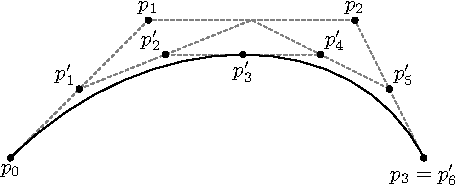
\includegraphics{subdivision}
% 	     \caption{A Figure}
% 	 \label{subd}
% 	\end{figure}

% \clearpage %% starts a new page and stops trying to place floats such as tables and figures

% \section{More Figure Stuff}
% You can also scale and rotate figures.
%  	\begin{figure}[h!]
	   
% 	       \centering
% 	    % DO NOT ADD A FILENAME EXTENSION TO THE GRAPHIC FILE
% 	    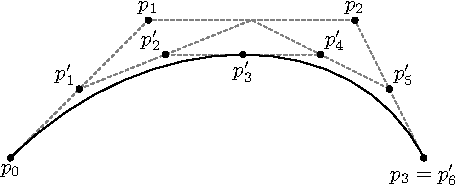
\includegraphics[scale=0.5,angle=180]{subdivision}
% 	    % if your figure shows up not where you want it, it may just be too big to fit. You can use the scale argument to shrink it, e.g. scale=0.85 is 85 percent of the original size. 
% 	     \caption{A Smaller Figure, Flipped Upside Down}
% 	 \label{subd2}
% 	\end{figure}

% \section{Even More Figure Stuff}
% With some clever work you can crop a figure, which is handy if (for instance) your EPS or PDF is a little graphic on a whole sheet of paper. The viewport arguments are the lower-left and upper-right coordinates for the area you want to crop.

%  	\begin{figure}[h!]
% 	    	       \centering
% 	    % DO NOT ADD A FILENAME EXTENSION TO THE GRAPHIC FILE
% 	   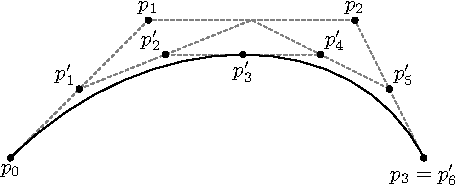
\includegraphics[clip=true, viewport=.0in .0in 1in 1in]{subdivision}
% 	    \caption{A Cropped Figure}
% 	 \label{subd3}
% 	\end{figure}
	
%       \subsection{Common Modifications}
%       The following figure features the more popular changes thesis students want to their figures. This information is also on the web at \url{web.reed.edu/cis/help/latex/graphics.html}.
%     %\renewcommand{\thefigure}{0.\arabic{figure}} 	% Renumbers the figure to the type 0.x
%     %\addtocounter{figure}{4} 						% starts the figure numbering at 4
%     \begin{figure}[htbp]
%     \begin{center}
%    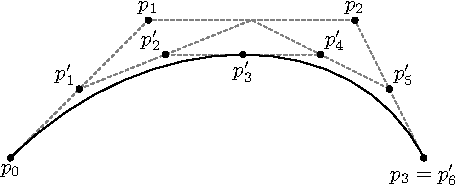
\includegraphics[scale=0.5]{subdivision}
%     \caption[Subdivision of arc segments]{\footnotesize{Subdivision of arc segments. You can see that $ p_3 = p_6^\prime$.}} %the special ToC caption is in square brackets. The \footnotesize makes the figure caption smaller
%     \label{barplot}
%     \end{center}
%     \end{figure} 

% \chapter*{Conclusion}
%          \addcontentsline{toc}{chapter}{Conclusion}
% 	\chaptermark{Conclusion}
% 	\markboth{Conclusion}{Conclusion}
% 	\setcounter{chapter}{4}
% 	\setcounter{section}{0}
	
% Here's a conclusion, demonstrating the use of all that manual incrementing and table of contents adding that has to happen if you use the starred form of the chapter command. The deal is, the chapter command in \LaTeX\ does a lot of things: it increments the chapter counter, it resets the section counter to zero, it puts the name of the chapter into the table of contents and the running headers, and probably some other stuff. 

% So, if you remove all that stuff because you don't like it to say ``Chapter 4: Conclusion'', then you have to manually add all the things \LaTeX\ would normally do for you. Maybe someday we'll write a new chapter macro that doesn't add ``Chapter X'' to the beginning of every chapter title.

% \section{More info}
% And here's some other random info: the first paragraph after a chapter title or section head \emph{shouldn't be} indented, because indents are to tell the reader that you're starting a new paragraph. Since that's obvious after a chapter or section title, proper typesetting doesn't add an indent there. 


%If you feel it necessary to include an appendix, it goes here.
    % \appendix
    %   \chapter{The First Appendix}
    %   \chapter{The Second Appendix, for Fun}


%This is where endnotes are supposed to go, if you have them.
%I have no idea how endnotes work with LaTeX.

  \backmatter % backmatter makes the index and bibliography appear properly in the t.o.c...

% if you're using bibtex, the next line forces every entry in the bibtex file to be included
% in your bibliography, regardless of whether or not you've cited it in the thesis.
    \nocite{*}

% Rename my bibliography to be called "Works Cited" and not "References" or ``Bibliography''
% \renewcommand{\bibname}{Works Cited}

%    \bibliographystyle{bsts/mla-good} % there are a variety of styles available; 
%  \bibliographystyle{plainnat}
% replace ``plainnat'' with the style of choice. You can refer to files in the bsts or APA 
% subfolder, e.g. 
% \bibliographystyle{annotate}  % or
% \bibliography{thesisdsldesktop}
 % Comment the above two lines and uncomment the next line to use biblatex-chicago.
 \printbibliography %[heading=bibintoc]

% Finally, an index would go here... but it is also optional.
\end{document}
